 % \documentclass[sigconf]{acmart}
\documentclass{article}
% We want page numbers on submissions

%%\ccsPaper{9999} % TODO: replace with your paper number once obtained

%packages
\usepackage{natbib}
\usepackage{amsmath}
\usepackage{amsthm}
\usepackage{mathtools}
\usepackage{mdframed}
\usepackage{subfigure}
\usepackage{booktabs}
% \usepackage{hyperref}
\usepackage{subfigure}
\usepackage{siunitx} % Provides the \SI{}{} and \si{} command for typesetting SI units
\usepackage{graphicx} % Required for the inclusion of images
% \usepackage{natbib} % Required to change bibliography style to APA
\usepackage{datetime}
\usepackage{lscape}
\usepackage{algorithm}
\usepackage{algorithmic}
\usepackage{xspace}
\usepackage[english]{babel} % English language/hyphenation
\usepackage{proof}
\usepackage{booktabs} % Top and bottom rules for tables
\usepackage[colorlinks, allcolors = blue,]{hyperref}
\usepackage{accents}
\usepackage{amsfonts}
\usepackage{stmaryrd}
\usepackage{amsmath,amsthm,amssymb,latexsym} 
\usepackage{microtype}
\usepackage{graphicx}
\usepackage{subfigure}
\usepackage{booktabs} % for professional tables
\usepackage{hyperref}
\usepackage{icml2019}
\usepackage{lipsum}

\usepackage{authblk}


%new commands
\newcommand{\theHalgorithm}{\arabic{algorithm}}
\newtheorem{definition}{Definition}
\usepackage{cancel}
\usepackage[normalem]{ulem}
\newcommand{\dataobs}{\textbf{x}}
\newcommand{\adj}[2]{\textbf{adj}(#1,#2)}
\newcommand{\candidateset}{\mathcal{R}_{\textup{post}}}
\newcommand{\bprior}{\boldsymbol{\beta}_{\textup{prior}}}
\newcommand{\bysinfer}{\mathsf{Infer}}
\newcommand{\betad}{\mathsf{Beta}}
\newcommand{\betaf}{\textup{B}}
\newcommand{\mbetaf}{\boldsymbol{\textup{B}}}
\newcommand{\vtheta}{\boldsymbol{\theta}}
\newcommand{\valpha}{\boldsymbol{\alpha}}
\newcommand{\vbeta}{\boldsymbol{\beta}}
\newcommand{\lapmech}{\mathsf{LSDim}}
\newcommand{\ilapmech}{\mathsf{LSHist}}
\newcommand{\binomial}[2]{\mathsf{Bin}(#1, #2)}
\newcommand{\multinomial}[2]{\mathsf{Mult}(#1, #2)}
\newcommand{\expmech}{\mathsf{EHD}}
\newcommand{\hexpmech}{\mathsf{EHDS}}
\newcommand{\lexpmech}{\mathsf{EHDL}}
\newcommand{\hexpmechd}{\mathsf{expMech}^{D}_{\hellinger}}
\newcommand{\privinfer}{\mathsf{PrivInfer}}
\newcommand{\hlg}{\mathsf{H}}
\newcommand{\dirichlet}[1]{\mathsf{Dir}(#1)}
\newcommand{\alphas}{\boldsymbol{\alpha}}
\newcommand{\xis}{\boldsymbol{\xi}}
\newcommand{\iverson}[1]{[#1]}
\newcommand{\datauni}{\mathcal{X}}
\newcommand{\hellinger}{\mathcal{H}}
\newcommand{\ux}[1]{u(\textbf{x}, {#1})}
\newcommand{\uxadj}[1]{u(\textbf{x}', {#1})}
\newcommand{\cardinality}[2]{\mathcal{C}^{#1}_{#2}}
\newcommand{\range}{\mathcal{O}}
\newcommand{\nomalizer}[1]{\sum\limits_{r'\in \mathcal{R}_{\textup{post}}} \exp \big(\frac{-\epsilon\cdot \mathcal{H} (\mathsf{BI}(#1),r')}{4 \cdot S(#1)}\big)}

\newcommand{\unomalizer}[1]{\sum\limits_{r'\in \mathcal{R}_{\textup{post}}} \exp \big(\frac{-\epsilon\cdot u(#1, r')}{4 \cdot S(#1)}\big)}


\newcommand{\hexpmechPr}[2]{\underset{z \thicksim \hexpmech(#1)}{\Pr}\left[ #2 \right]}
\newcommand{\lapmechPr}[2]{\underset{z \thicksim \lapmech(#1)}{\Pr}\left[ #2 \right]}

\newcommand{\ilapmechPr}[2]{\underset{
{z \thicksim \ilapmech(#1)}
}{\Pr}\left[ #2 \right]}

\newtheorem{thm}{Theorem}[section]

\newtheorem{lem}{Lemma}[section]

\newtheorem{assert}{Assertion}[lem]
\newcommand{\lap}[2]{\mathsf{Lap}(#1, #2)}
\newcommand{\todo}[1]{{\footnotesize \color{red}\textbf{[[ #1 ]]}}}
\icmltitlerunning{Exploring the Design Space of Differentially Private
  Bayesian Inference under Hellinger Distance}

\begin{document}

\twocolumn[
\icmltitle{Exploring the Design Space of Differentially Private
  Bayesian Inference under Hellinger Distance}

% It is OKAY to include author information, even for blind
% submissions: the style file will automatically remove it for you
% unless you've provided the [accepted] option to the icml2019
% package.

% List of affiliations: The first argument should be a (short)
% identifier you will use later to specify author affiliations
% Academic affiliations should list Department, University, City, Region, Country
% Industry affiliations should list Company, City, Region, Country

% You can specify symbols, otherwise they are numbered in order.
% Ideally, you should not use this facility. Affiliations will be numbered
% in order of appearance and this is the preferred way.
\icmlsetsymbol{equal}{*}

\begin{icmlauthorlist}
\icmlauthor{Jiawen Liu}{to}
\icmlauthor{Gian Pietro Farina}{to}
\icmlauthor{Tetsuya Sato}{to}
\icmlauthor{Mark Bun}{ed}
\icmlauthor{Marco Gaboardi}{to}
\end{icmlauthorlist}

\icmlaffiliation{to}{Department of Computer Science and Engineering, University at Buffalo, SUNY, New York, United States}
\icmlaffiliation{ed}{Princeton University, United States}

% \icmlcorrespondingauthor{Cieua Vvvvv}{c.vvvvv@googol.com}
% \icmlcorrespondingauthor{Eee Pppp}{ep@eden.co.uk}

% You may provide any keywords that you
% find helpful for describing your paper; these are used to populate
% the "keywords" metadata in the PDF but will not be shown in the document
\icmlkeywords{Machine Learning, ICML}

\vskip 0.3in
]

\printAffiliationsAndNotice{\icmlEqualContribution} % otherwise use the standard text.

\begin{abstract}
% Several approaches have been explored in order to make Bayesian inference
% differentially private.
% For instance, \cite{dimitrakakis2014robust} and
% \cite{wang2015privacy} proved that, under specific conditions of the likelihood function and the prior distribution,
% sampling from the posterior distribution, is already differentially private. \cite{zhang2016differential} and \cite{foulds2016theory}
% designed differentially private (d.p.) mechanisms by adding laplacian noise
% to the numeric parameters of the posterior distributions. 
% Accuracy, is usally (\cite{??}) measured by providing upper bounds, holding w.h.p, on the
% $\ell_1$ or $\ell_\infty$-distance between the numeric parameters
% of the released posterior distribution and the actual real ones of posterior distribution.
We explore the design space of differentially private Bayesian
inference mechanisms with accuracy measured in terms of the Hellinger
distance between posterior distributions.  
We focus on two discrete models for parametric Bayesian
inference: the Beta-Binomial and the Dirichlet-Multinomial
models. We study two mechanisms based on 
Laplace perturbation of the parameters of the posterior distribution under the
$\ell_1$ norm, and compare them with a discrete mechanism
calibrating noise to a smooth upper bound on the Hellinger distance.
Accuracy is measured through the Hellinger distance between the posterior
distribution released by a given mechanism and the one obtained via non-private inference.
We compare the accuracy of our mechanisms theoretically and experimentally.
\end{abstract}
 % TODO: replace with your keywords





\section{Introduction}
\label{sec_intro}
%%Data analysis and privacy are important
Modern data analysis techniques have enabled significant advances in a
variety of applications in medicine, finance, social science, and transportation.
In order to provide better services, these applications need large amounts of users' data,
putting at risk the privacy of individual users contributing their data. 
Differential privacy was proposed a decade ago to address privacy concerns
in these situations, and is now the standard for privacy-preserving data analysis.
 %and it is on its way to become the gold standard in data
%privacy.  

%%Bayesian inference is a standard tool for data analysis which is
%% also a building block of probabilistic programming languages
Many statistical applications are driven by Bayesian inference.
This is a standard statistical tool in which a prior distribution is combined
with a sample of observed data in order to estimate a new posterior distribution.


%is a standard statistical tool that is useful to
%estimate a posterior distribution when a prior distribution is given
%and some data is observed. 

%%Several works have considered differentially private bayesian
%%inference 

%%we consider bayesian inference with posterior perturbation 
%%which could be used as a plug and play in PPL citing CCS2016


In this work we consider the design space of  parametric Bayesian
inference mechanisms guaranteeing differential privacy. Our work is
motivated by recent developments in the area of probabilistic
programming where several tools have been proposed to perform
parametric and non-parametric Bayesian inference in an efficient
way.


%%we focus on discrete simple models

%%we focus on hellinger distance

%%the contribution is a comparative study of several ways to achieve
%%differential privacy in this setting.

%%findings: Laplace with histogram is the best mechanism and this is
%%because when the data size grows the hellinger between the
%%posteriors induced by adjacent datasets decreases, and so the impact
%%of Laplace also decreases. This is a particular case because of the
%%hellinger, if the Laplace is added accordingly to the dimension the
%%performance is worse. The exponential with smooth sensitivity is
%%better than the standard exponential with global sensitivity but it
%%does not achieve the same performance as the previous ones. 

We focus on inference tasks based on two classical statistical models: the Beta-Binomial and the
Dirichlet-Multinomial models. In the Beta-Binomial model, we are given a
dataset consisting of independent Bernoulli trials with bias $p$. Given an initial
prior belief that $p$ follows a Beta distribution, we may use the dataset to infer a
posterior belief that $p$ follows a Beta distribution with updated parameters. This model
generalizes to the Dirichlet-Multinomial model, in which a multinomial distribution
is used to describe categorial data with more than two possible outcomes. Similarly, the goal
is infer a belief about the proportions of each outcome. Given a prior belief that these proportions
come from a Dirichlet distribution, the posterior belief given multinomial data will
also follow a Dirichlet distribution.

%
%In the Beta-Binomial model the goal
%is to estimate an unknown fraction of a population from a sequence
%of Bernoulli trials each of which is either 0 or 1 and from an initial
%prior belief, a Beta distribution, on that fraction; the trials are assumed to be independent
%given the value of the bias. In the Dirichlet-Multinomial model a Multinomial
%distribution is used to describe categorical data with more than
%two possible outcomes. Similarly, the aim is to learn the various
%unknown proportions of a population from a sequence of trials
%each of which having more than two possible outcomes. Again,
%a prior belief, a Dirichlet distribution, is used to describe the initial knowledge
%about those fractions. The posterior distributions on the proportions will be
%respectively a Beta distribution and a Dirichlet distribution.


In our work, we consider mechanisms which output a complete description of the posterior
distribution inferred using private data.
While the prior distribution associated to a given inference task is considered public information,
the inferred posterior distribution may leak information about the individuals in the dataset.
In order to guarantee differential privacy, we introduce random noise to the posterior before releasing it.
Our goal is to design mechanisms which are accurate, in the sense that this noisy posterior is close
to the posterior one would have inferred without concern for privacy. The most natural way
to measure closeness is via a distance between probability distributions -- nevertheless, only a few works 
in the literature (e.g., \cite{zhang2016differential}) actually state accuracy guarantees in this way.






The amount of the noise that we need to introduce
depends on the differential privacy parameter $\epsilon$ and the sensitivity of the inference to
small changes in the input dataset.
As with accuracy, sensitivity may be measured in many different ways, with each choice giving rise to a different
method of introducing noise for differential privacy.
%Sensitivity can be computed in many different ways based on which metric space
%we consider on the output space of the mechanism. 
In the existing literature on private Bayesian
inference (e.g. \cite{zhang2016differential,xiao2012bayesian}), sensitivity is measured via a norm (e.g., the $\ell_1$ norm)
on the the vector of numbers parametrizing the output distribution. But when the accuracy of a mechanism is determined by
a distance on distributions themselves, this may not be such a natural choice. The distance between
two parameterized distributions may behave wildly as a function of the distance between the vectors of parameters characterizing them.

A more natural approach, which we propose here, is to also directly measure sensitivity with respect
to a metric on the space of inferred probability distributions. Our goal is to identify cases where jointly measuring
accuracy and sensitivity in terms of a single metric on probability distributions can yield improved accuracy. 
{\color{red}{MB: Is this accurate? Would we ever want to use different metrics for accuracy and sensitivity?}}


%A more natural approach which we explore here, is to measure sensitivity with respect to
%a metric on the space of inferred probability distributions.
%Another question is that of how to measure accuracy. Again,
%this can be answered in different ways based on the metric
%imposed on the output space, and yet again
%only in few works in literature (e.g. \cite{zhang2016differential})
%distances between probability measures have been used for these purposes.


%The question that this work aims at answering is whether
%an approach based on probability metrics can improve on
%the accuracy of approaches based on metrics over
%the numeric parameters of the distributions. 
%We will see that in some cases this can happen.

%\noindent \textbf{Main contributions.}
In summary, the main contributions of our work are:
\begin{itemize}
	\item We give a new differentially private Bayesian inference mechanism based on the standard exponential mechanism.
   %    \item A full proof of $(\epsilon, \delta)$-differential privacy of the mechanism is given in the paper. 
	\item We propose two ways of improving the accuracy of this basic mechanism: 1) We calibrate noise to a measure of sensitivity determined by a metric between distributions
      (e.g. Hellinger distance ($\hellinger$), $f$-divergences, etc\dots). 2) We scale noise according to a a smooth upper bound on the local sensitivity, rather than according to global sensitivity.
  \item We implement the new proposed mechanism and other art-of-state mechanisms, comparing their performances in terms of accuracy and privacy.
\end{itemize}

\section{Related Work}

% A plentiful of data analysis algorithms have been studied to preserve differential privacy, including the subspace clustering algorithm \cite{wang2015differentially}, the gradient decedent algorithm in deep learning \cite{abadi2016deep}, logical regression \cite{chaudhuri2009privacy}, principle component analysis \cite{chaudhuri2012near}, probabilitic inference \cite{williams2010probabilistic} and convergence in statistic estimation \cite{chaudhuri2012convergence}, etc. 

Several works have considered the intersection of Bayesian Inference and differential
privacy. \citet{williams2010probabilistic} explored the use of
probabilistic inference to improve the accuracy of differentially
private data analyses. A similar approach has been also studied by
\citet{xiao2012bayesian}.


A general trend has been to study robustness conditions
for different likelihood functions and different classes of conjugate priors 
guaranteeing differential privacy for samples taken from a
posterior distribution. \citet{dimitrakakis2014robust}
consider this approach and identify some general robustness technique
which can be applied to several models including the one considered in
this paper. Similarly, \citet{zheng2015differential} considers a similar approach
but with different conditions. \citet{zhang2016differential} extend
the previous approaches to address more general models with multiple
random variables. 
\citet{wang2015privacy} identifies
conditions guaranteeing differential privacy for samples generated
using standard montecarlo algorithm.
\citet{GeumlekSC17} consider the problem of releasing samples from
distributions in the exponential family under the constraints imposed
by Renyi differential privacy. 
\citet{Zhang2017privbayes} propose a technique for releasing high
dimensional data based on the differentially private learning of a
Bayesian graphical model. 

Few works take an approach similar to the one we consider here. 
\citet{dimitrakakis2015differential} study differentially private
posterior release by output perturbation based on Laplace noise for the Beta-Binomial
model. However, they measure accuracy in terms of $\ell_1$
distance over the parameters and in term of KL-divergence over the distribution.  \citet{foulds2016theory}
generalizes the approach of \citet{dimitrakakis2015differential} by
analyzing further the impact that Laplace noise has on the inference.
They also focus on accuracy measured in term of  $\ell_1$ distance
over the parameters. \citet{BartheFGAGHS16} study a verification
method for probabilistic programs including constructs for Bayesian
inference. In their work they also study an approach based on the use
of the exponential mechanism with the Hellinger distance as scoring
function. We show here that their approach achieve very poor utility. 


% 3) The inference process is differentially private and the posterior distribution released should be private itself, in the meantime, with good accuracy. The third topic where our work focus on is still very new. moreover, their design spaces are more specific to the $\ell_1$ norm and Laplace mechanism. That's why we explore different metrics and different algorithms over the design space.


\section{Preliminaries}
\label{sec_background}
\noindent \textbf{Bayesian inference.} 
Given a prior belief $\Pr(\theta)$ on some parameter $\theta$,
and an observation $\dataobs$, the posterior distribution on $\theta$
given $\dataobs$ is defined by Bayes' Theorem as:
\[
  \Pr(\theta | \dataobs) = \frac{\Pr(\dataobs | \theta) \cdot \Pr(\theta)}{\Pr(\dataobs)}
\]
where the expression $\Pr(\dataobs | \theta)$ denotes the
\emph{likelihood} of observing $\dataobs$ under a value of
$\theta$. 
% Since we consider $\dataobs$ to be fixed, the likelihood is
% a function of $\theta$.
% For the same reason $\Pr(\dataobs)$ is a constant independent of $\theta$.
% Usually in statistics the prior distribution $\Pr(\theta)$ is chosen so that it represents
% the initial belief on $\theta$, that is, when no data has been
% observed. In practice though,
In parametric statistics, prior distributions and likelihood functions are usually chosen so that the posterior
belongs to the same \emph{family} of distributions as the prior. In this case we say that the prior
is conjugate to the likelihood function. Use of a conjugate prior
simplifies calculations and allows for inference to be performed in a
recursive fashion over the data. This approach is implemented in a
precise or approximate way in the compiler of several
probabilistic programming languages~\cite{}.

%  support bayesian inference
% by means of a language primitive, often called $\bysinfer$, which
% supports the (precise or approximate) parametric computation of the
% posterior of a given model. In the rest of the paper, we will use the following
% notation as a shorthand for the inference process:
% \[
%   \bysinfer(\Pr(\dataobs | \theta), \Pr(\theta), \dataobs) = \frac{\Pr(\dataobs | \theta) \cdot \Pr(\theta)}{\Pr(\dataobs)}
% \]
\noindent \textbf{Dirichlet-multinomial model.}
In this work we will focus on the Dirichlet-Multinomial model for
categorical data and its restriction to binary data: the Beta-Binomial
model. 
That is, we will consider the situation where 
the underlying categorical data is drawn from a multinomial
distribution with parameter the vector $\vtheta\in [0,1]^{k}$. The prior distribution over $\vtheta$
is given by a Dirichlet distribution, $\dirichlet{\valpha}$, for,
$\valpha\in(\mathbb{R}^{+})^{k}$ and $k\in\mathbb{N}$, with p.d.f:
\[
\Pr(\vtheta)=\frac{1}{\mbetaf(\valpha)}\cdot\prod_{i=1}^{k}{\theta_i^{\alpha_i-1}}
\]
where $\mbetaf(\cdot)$ is the generalized beta function.
The data $\dataobs$ is a sequence of $n\in\mathbb{N}$ values
coming from a universe $\datauni$, such that $|\datauni|=k$.
The likelihood function is
$
\Pr(\dataobs|\vtheta)=\prod_{a_i\in\datauni}\theta_{i}^{\Delta \alpha_i},
$
with $\Delta \alpha_i=\displaystyle\sum_{j=1}^{n}\mathbf{1}_{\iverson{x_j=a_i}}$.
Denoting by $\Delta\valpha$ the vector $(\Delta\alpha_1,\dots
\Delta\alpha_k)$ the posterior distribution over $\vtheta$ is
$\dirichlet{\valpha + \Delta \valpha}$, where $+$ denotes the componentwise sum of vectors.
In the following we will use the notation $\bysdir(n,\vtheta, \valpha,
\dataobs)$ to denote the posterior of this process.
%i.e., $\bysdir(n,\vtheta, \valpha, \dataobs)=\dirichlet{\valpha + \Delta \valpha}$.
%
% ($\thicksim \binomial{n}{\theta}$), where $\theta$ represents
% the parameter --informally called \emph{bias}-- of a Bernoulli
% distributed random variable and $n$ is the number of draws. The
% prior distribution over $\theta\in [0,1]$ is going to be a beta
% distribution, $\betad(\alpha, \beta)$, with parameters
% $\alpha,\beta\in\mathbb{R}^{+}$, and with p.d.f:
% \[
%   \Pr(\theta)= \frac{\theta^{\alpha} (1- \theta)^{\beta}}{\betaf(\alpha,\beta)}
% \]
% where $\betaf(\cdot,\cdot)$ is the beta function.
% The data $\dataobs$ will be a sequence of $n\in\mathbb{N}$ binary values, that is $\dataobs= (x_1,\dots x_n), x_i\in\{0,1\}$, and the likelihood function is:
% \[
%   \Pr(\dataobs | \theta)= \theta^{\Delta \alpha}(1-\theta)^{n - \Delta \alpha}
% \]
% where $\Delta \alpha = \sum_{i=1}^{n}x_i$.
% The posterior distribution over $\theta$ can be easily proven to be equal to:\[\betad(\alpha + \Delta \alpha,\beta + n - \Delta \alpha)\]
% From now on we will denote by $\bysinfer(\binomial{n}{\theta}, \betad(\alpha, \beta), \dataobs)$ the previous
% posterior distribution. This notation will prove itself handy when its arguments will change types in the next example and
% in section \ref{} when the private mechanisms will be described.

% We will consider the situation where the underlying data is drawn from a binomial distribution
% ($\thicksim \binomial{n}{\theta}$), where $\theta$ represents
% the parameter --informally called \emph{bias}-- of a Bernoulli
% distributed random variable and $n$ is the number of draws. The
% prior distribution over $\theta\in [0,1]$ is going to be a beta
% distribution, $\betad(\alpha, \beta)$, with parameters
% $\alpha,\beta\in\mathbb{R}^{+}$, and with p.d.f:
% \[
%   \Pr(\theta)= \frac{\theta^{\alpha} (1- \theta)^{\beta}}{\betaf(\alpha,\beta)}
% \]
% where $\betaf(\cdot,\cdot)$ is the beta function.
% The data $\dataobs$ will be a sequence of $n\in\mathbb{N}$ binary values, that is $\dataobs= (x_1,\dots x_n), x_i\in\{0,1\}$, and the likelihood function is:
% \[
%   \Pr(\dataobs | \theta)= \theta^{\Delta \alpha}(1-\theta)^{n - \Delta \alpha}
% \]
% where $\Delta \alpha = \sum_{i=1}^{n}x_i$.
% The posterior distribution over $\theta$ can be easily proven to be equal to:\[\betad(\alpha + \Delta \alpha,\beta + n - \Delta \alpha)\]
% From now on we will denote by $\bysinfer(\binomial{n}{\theta}, \betad(\alpha, \beta), \dataobs)$ the previous
% posterior distribution. This notation will prove itself handy when its arguments will change types in the next example and
% in section \ref{} when the private mechanisms will be described.
% \noindent \textbf{Dirichlet-multinomial Systems.}
%
The Beta-Binomial model can be obtained from the Dirichlet-Multinomial
model by fixing $k=2$. 

\noindent \textbf{Hellinger distance.}
The \emph{Hellinger} distance $\hellinger(\cdot,\cdot)$ is a statistical
divergence measuring the distance between two probability
distributions. Given two probability distributions $\textup{P}$ and $\textup{Q}$,
the Hellinger distance between them is defined as:
\[
\hellinger(P,Q) =\sqrt{\frac{1}{2} \int \bigg(\frac{dP}{d \lambda} - \frac{dQ}{d \lambda}\bigg)^2 d \lambda}
\]
When we consider the Hellinger distance between Dirichlet
distributions we can simplify this definition to close form. If $\textup{P}=\dirichlet{\valpha_1}$ and
$\textup{Q}=\dirichlet{\valpha_2}$ we have: 
 \[
   \hellinger(\dirichlet{\valpha_1}, \dirichlet{\valpha_2}) = \sqrt{1 - \frac{\betaf(\frac{\valpha_1 + \valpha_2}{2})}{\sqrt{\betaf(\valpha_1) \betaf(\valpha_2)}}}
 \]

\noindent \textbf{Differential Privacy.}
\emph{Differential privacy}~\cite{dwork2006} is a quantitative notion
of data privacy guaranteeing  a bound on the that changing the input of a mechanism slightly only reflects
in a controlled and bounded way on the output distribution. 
Formally, the $\epsilon$ parameter
controls how much two outputs starting from \emph{close} inputs can differ. When two inputs are close we call them \emph{adjacent}.
By adjacency we usually mean a relation over input databases which includes all the pair of databases which differ by at most one row.
The formal definition of $\epsilon$-differential privacy follows.
\begin{definition}
\label{def_epsilon_dp}

A randomized mechanism $\mathcal{M}$ with domain $\mathbb{N}^{|\mathcal{X}|}$ and codomain $\range$, is $\epsilon$-differential private, if for all adjacent
\footnote{Given $\dataobs, \dataobs'\in\{0,1\}^n$  we say that $\dataobs$ and $\dataobs'$ are adjacent and we write, iff
$\sum_{i}^{n}\iverson{x_i = x'_i }\leq 1$. } $\dataobs, \dataobs' \in \mathbb{N}^{|\mathcal{X}|}$ and all $\mathcal{S} \subseteq \range$:
\begin{equation*}
\Pr[\mathcal{M}(\dataobs) \in \mathcal{S}] \leq e^\epsilon \Pr[\mathcal{M}(\dataobs') \in \mathcal{S}].
\end{equation*}

\end{definition}


It is possible to achieve $\epsilon$-differential privacy through use and composition of
a few basic components. Some of these components are now reviewed.

\noindent \emph{Laplace mechanism.}
The Laplace mechanism releases a random number drawn from the Laplace distribution with
mean $\mu=q(d)$ and scale $\nu$. Where $q$ is a numeric query on a database $d$.
If $\nu\geq \frac{\Delta_f}{\epsilon}$, with $\Delta_f=\displaystyle\max_{d,d':\adj{d}{d'}}{\lvert f(d_1)-f(d_2)\lvert}$
then the mechanism is $\epsilon$-differentially private as proven in \cite{???}.

\noindent \emph{Exponential mechanism.}
 
\noindent \emph{Composition.}

\noindent \emph{Postprocessing.}

\noindent \emph{A note on input data representation.}
We will think of our input databases $\dataobs$ of length $n$ as histograms 
with $k$-$1$ bins where $k$ is the dimensionality of the problem.
This is w.l.o.g. because given the first $k$-$1$ counts, the $k$-th count
is known.

\section{Problem Statement}
\label{subsec_problem}
We are interested in exploring the design space of mechanisms for privately releasing the posterior
distribution for the Dirichlet-Multinomial model by output
perturbation with accuracy measured in Hellinger distance. We assume
that the prior is given and non-private and we aim at protecting the
privacy of the observed data.
It is worth noticing that the posterior distribution of the Dirichlet-Multinomial model is fully characterized
by its parameters. That is, we are interested in releasing a private version of
the Dirichlet distribution with parameter
$\valpha'=(\valpha + \Delta \valpha)$, where $\valpha$ is the
parameter of the prior, and $\Delta \valpha$ is computed from the data
as discussed in the previous section. In the case of the
Beta-Binomial model this specialize to releasing a private version of the Beta distribution with 
parameters $(\alpha',\beta')=(\alpha + \Delta \alpha,\beta + n -
\Delta \alpha)$, where $\alpha$ and $\beta$ are the parameters of the
prior, and $\Delta \alpha$ is the number of $1$ in the data.


Previous work by \citet{zhang2016differential} and \citet{xiao2012bayesian}
have considered the problem of releasing the posterior of the
Beta-Binomial model by output perturbation with accuracy measured in terms of
$\ell_1$ norm. In addition,  \citet{zhang2016differential} has also
considered KL-divergence between posteriors. 
In this work we consider instead the Hellinger distance between
posteriors. Similarly to KL-divergence, Hellinger distance is an
$f$-divergence measuring levels of similarities between
distributions. However, unlikely KL-divergence, Hellinger distance is a proper
distance satisfying reflexivity, symmetry and triangle
inequality. These properties gives Hellinger distance analytical
advantages and makes the minimum hellinger distance  an efficient and
robust estimator~\cite{}.


% attacked this problem by adding independent Laplacian noise to the
% parameters of the posteriors. That is, in the case of the Beta-Binomial system,
% the values released would be: $(\tilde\alpha,\tilde\beta)=(\alpha +  \widetilde{\Delta \alpha},\beta + n - \widetilde{\Delta \alpha})$
% where $\widetilde{\Delta \alpha}\thicksim \lap{\Delta \alpha}{\frac{2}{\epsilon}}$,
% and where $\lap{\mu}{\nu}$ denotes a Laplace random variable with mean $\mu$ and scale $\nu$.
% This mechanism is $\epsilon$-differentially private, and the noise is
% calibrated w.r.t. to a sensitivity of 2 which is derived by using
% $\ell_1$ norm over the pair of parameters. Indeed, considering two
% adjacent data observations $\dataobs, \dataobs'$, that, from a unique prior, give rise to two posterior
% distributions, characterized by the pairs
% $(\alpha',\beta')$ and $(\alpha'',\beta'')$ then
% $|\alpha'-\alpha''|+|\beta'-\beta''|\leq 2$.
% This argument extends similarly to the Dirichelet-Multinomial system. Details are introduced in Section \ref{sec_mechs}.\\
% However, in previous works, the accuracy of the posterior was measured with respect to $\ell_1$ norm. That is, an upper bound was given on
% \[
%   \Pr[|\alpha - \tilde\alpha| + |\beta - \tilde\beta |\geq \gamma ]
% \]
% where $(\alpha, \beta), (\tilde\alpha,\tilde\beta)$ are the real and the perturbed pairs of parameters, respectively.
% However, distance between
% distributions are more naturally  measured by distribution
% metrics such as $f$-divergences, e.g. Hellinger distance, etc., than the $\ell_1$ norm shown above.
% {\color{blue} still not sure this is a good way to put it...}
% This gives us motivation for exploring the design space
% of mechanisms by considering different norms. e.g. a norm over space of measures.
% to compute the sensitivity and provide guarantees on the accuracy.

One of the challenges in working with the Hellinger distance for the
Dirichlet-multinomial model is that a difference in the parameters of two
Dirichlet distributions can results in different values  in terms of Hellinger distance
depending on the value of the parameter
themselves. The plot in Figure~\ref{fig_sensitivity} illustrates
this by showing the Hellinger distance between beta distributions
whose parameters differ by one, for each value of the parameter
$\alpha$. The reason why this change is relevant
for differential privacy is that this quantity corresponds to the local
sensitivity of the function $\hellinger$. 


\begin{figure}[ht]
\centering
\includegraphics[width=0.32\textwidth]{sensitivity_2d.eps}
\caption{Hellinger distance between the Beta distributions
  corresponding to two adjacent datasets of size 100
  when  $\alpha$ (the number of 1s) changes. This quantity corresponds
  to the local sensitivity of the function $\hellinger$.}
\label{fig_sensitivity}
\end{figure}



\section{Private Mechanisms}
\label{sec_mechs}
In this section we will describe and analyse a series of mechanisms to privately compute and release
a posterior distribution.
Section \ref{sec_ell1_dim} presents a first mechanism, $\lapmech$,
based on the Laplace primitive where the sensitivity is measured w.r.t. to $\ell_1$ norm.
Section \ref{sec_ell1_hist}, shows that $\lapmech$'s accuracy can be improved
by performing a better analysis on the sensitivity of the inference process.
Section \ref{sec_ehd}, shows an instance of the exponential mechanism, $\expmech$, where the scoring
function is based on the Hellinger distance, we will see how this mechanisms performs
poorly due to the very high global sensitivity of the inference process w.r.t to this metric.
We then proceed to introduce $\lexpmech$, a variation of $\expmech$ which uses a lower bound
on the global sensitivity called local sensitivity.
Unfortunately, despite improving on accuracy $\lexpmech$ is non-private.
Finally, building on $\lexpmech$, we introduce $\hexpmech$:
which, based on the notion of \emph{smooth} sensitivity, achieves $\epsilon$-differential privacy and
has good accuracy in specific cases.
In presenting these mechanisms we will denote by $\inferd{\valpha}{\vtheta}{\dataobs}$ the posterior  $\dirichlet{\valpha'}$
obtained starting from the prior $\dirichlet{\valpha}$, likelihood $\multinomial{|\dataobs|}{\vtheta}$, and observed data $\dataobs$.
To minimize notation we will identify the distribution $\dirichlet{\valpha}$ with its vector
of parameters.
Two different upper bounds to the value of
\begin{align}
  \label{eqn:eq1}
  \max_{\substack{\adj{\dataobs}{\dataobs'},\\
      \valpha=\inferd{\valpha}{\vtheta}{\dataobs},\\
      \valpha'=\inferd{\valpha}{\vtheta}{\dataobs'}}}||\valpha-\valpha'||_1 
\end{align}
will be used to calibrate the noise in the mechanisms based on the Laplacian primitive.
Finally, with $\bys{\dataobs}{\vtheta}$ we will denote $\inferd{\valpha}{\vtheta}{\dataobs}$ when no confusion can arise.



\subsection{Calibrating noise w.r.t. $\ell_1$ norm ($\lapmech$)}
\label{sec_ell1_dim}
We start off by presenting $\lapmech$, in Algorithm \ref{lapmech}, based on the Laplace primitive.
The idea of $\lapmech$ is to add Laplacian noise with scale proportional to $\mathcal{X}$ to
the differences between the respective numeric parameters of the prior
and posterior distribution. 
\begin{algorithm}
  \caption{$\lapmech$}
  \label{lapmech}
  \begin{algorithmic}
  \INPUT $\dataobs\in\mathcal{X}^n$, $\dirichlet{\valpha}$
  \STATE \quad {\bf let} $\valpha' = \inferd{\valpha}{\vtheta}{\dataobs}$
  \STATE \quad {\bf Initialize} a vector $\tilde{\valpha} = (0, \dots, 0 )\in \mathbb{N}^{|\mathcal{X}|}$ 
  \STATE \quad {\bf For} $i = 1 \dots |\mathcal{X}| - 1$:
  \STATE \quad \quad  {\bf let} $\eta \sim \lap{0}{\frac{|\mathcal{X}|}{\epsilon}}$
  \STATE \quad \quad  $\tilde{\alpha_i}=\alpha_i + \lfloor{(\alpha_i' - \alpha_i) + \eta}\rfloor^n_0$ 
  % \RETURN $a_{k+1}$.
  \STATE \quad $\tilde{\alpha_{|\mathcal{X}|}} = \alpha_{|\mathcal{X}|} + \lfloor n - \sum_{i = 1}^{|\mathcal{X}|-1}\lfloor{(\alpha_i' - \alpha_i) + \eta_i}\rfloor^n_0 \rfloor^n_0$
  \STATE {\bf return} $\tilde{\valpha}$
  \end{algorithmic}
\end{algorithm}
\begin{lem}
  Algorithm \ref{lapmech} is $\epsilon$-d.p.
  \begin{proof} By noticing that $\mathcal{X}-1$ is an upper bound to the value denoted by (\ref{eqn:eq1}). \end{proof}
\end{lem}


\subsection{Improving the sensitivity ($\ilapmech$)}
\label{sec_ell1_hist}
By seeing the parameters of the distributions as histograms, we can give a tighter upper bound to the value denoted by (\ref{eqn:eq1}).
Indeed a constant will do. Algorithm $\ilapmech$ in Algorithm \ref{ilapmech} takes advantage of this fact. 
Indeed, when $\mathcal{X}=2$, 1 is an upper bound for the value of (\ref{eqn:eq1}), while when $\mathcal{X}>2$, 2 is.
In Algorithm \ref{ilapmech} the algorithm $\ilapmech$ is presented.
\begin{algorithm}
  \caption{$\ilapmech$}
  \label{ilapmech}
  \begin{algorithmic}
  \INPUT $\dataobs\in\mathcal{X}^n$, $\dirichlet{\valpha}$
  \STATE \quad {\bf let} $\valpha' = \inferd{\valpha}{\vtheta}{\dataobs}$
  \STATE \quad ${\bf let}\ k=\left \{
        \begin{array}{lll}          
          1&\text{if}& |\mathcal{X}|=2\\
          2&\text{otherwise}
        \end{array}
      \right .\ $
  \STATE \quad {\bf Initialize} a vector $\tilde{\valpha} = (0, \dots, 0 )\in \mathbb{N}^{|\mathcal{X}|}$ 
  \STATE \quad {\bf For} $i = 1 \dots |\mathcal{X}|-1$:
  \STATE \quad \quad  {\bf let} $\eta \sim \lap{0}{\frac{k}{\epsilon}}$
  \STATE \quad \quad  $\tilde{\alpha_i}=\alpha_i + \lfloor{(\alpha_i' - \alpha_i) + \eta}\rfloor^n_0$ 
  % \RETURN $a_{k+1}$.
  \STATE \quad $\tilde{\alpha_{|\mathcal{X}|}} = \alpha_{|\mathcal{X}|} + \lfloor n - \sum_{i = 1}^{|\mathcal{X}|-1}\lfloor{(\alpha_i' - \alpha_i) + \eta_i}\rfloor^n_0 \rfloor^n_0$
  \STATE {\bf return} $\tilde{\valpha}$
  \end{algorithmic}
\end{algorithm}
\begin{lem}
  Algorithm \ref{ilapmech} is $\epsilon$-d.p.
  \begin{proof} By noticing that 1 and 2 are upper bounds to the value denoted by (\ref{eqn:eq1}), respectively when $|\mathcal{X}|=2$ and $|\mathcal{X}|>2$.
  \end{proof}
\end{lem}

\subsection{A new family of mechanisms}
\label{sec_exp}
In this section, we explore  mechanism which we denote by $\expmech$. $\expmech$ is an instance
of the exponential mechanism \cite{talwar} where the scoring function is based on a metric over
probability distributions.
The idea is that $\expmech$ will sample and output a distribution with higher probability when
it is closer to the real posterior; importantly,  \emph{closer} is measured using a metric over probability
distributions as opposed to a metric over the parameters that represent it. In this work we will
use the Hellinger distance, but this approach could be extended to other $f$-divergences. 
Given a prior distribution $\dirichlet{\valpha}$,
we define the follwing set  where the mechanism will sample from:
\[
  \candidateset{\valpha}=\{\inferd{\valpha}{\vtheta}{\dataobs}\mid \dataobs \in \mathcal{X}^n\}.
\]
In general $|\candidateset{\valpha}|=\binom{n + 1}{|\mathcal{X}| - 1}$ when $\valpha\in\mathcal{X}^n$. In the specific case of $|\mathcal{X}|=2$ with $\valpha=(\alpha,\beta)$,
that is the Beta-Binomial model, the above reduces to:
\[
  \{(\alpha',\beta')\mid \alpha'=\alpha + \Delta\alpha, \beta'=\beta + n-\Delta\alpha,  \Delta\alpha=\sum x_i, \dataobs\in \{0,1\}^n\}
\]

\noindent \textbf{A first approach: the $\expmech$ mechanism.}
\label{sec_ehd}
$\expmech$'s pseudocode is shown in Algorithm \ref{mech:expmech1}. $\expmech$ is an instance
of the Exponential mechanism where the scoring function is instantiated with the function: $r\mapsto -\hellinger(\bysinfer{\dataobs}, r)$.
Given the input $\dataobs\in\mathcal{X}^n$ and a prior $\dirichlet{\valpha}$, the mechanism $\expmech$ outputs an element $r\in\candidateset{\valpha}$ with  probability: 
\[
\frac
  {\exp(\frac{-\epsilon\cdot \hellinger(\bys{\dataobs}{\valpha}, r)}{2\cdot GS})}
{\Sigma_{r' \in \candidateset{\valpha}}\exp(\frac{-\epsilon\cdot \hellinger(\bys{\dataobs}{\valpha}, r')}{2\cdot GS})},
\]
where $GS$ is the global sensitivity of the scoring function, defined as:
\[
\max_{\dataobs,\dataobs': \\ \adj{\dataobs}{\dataobs'}}\max_{r\in \candidateset{\valpha}}
|\hellinger(\bys{\dataobs}{\valpha}, r) - \hellinger(\bys{\dataobs'}{\valpha}, r)|
\]
% 
  \begin{algorithm}
  \caption{$\expmech$}
  \label{mech:expmech1}
  \begin{algorithmic}
  \INPUT observed data set $\dataobs \in \mathcal{X}^n$, prior: $\dirichlet{\valpha}$, $\epsilon$
  \STATE \quad {\bf let} $\dirichlet{\valpha'}= \bys{\dataobs}{\valpha}$.   
  \STATE \quad {\bf set} $z=r$ with probability $\frac
  {\exp(\frac{-\epsilon\cdot \hellinger(\bys{\dataobs}{\valpha}, r)}{2\cdot GS})}
{\Sigma_{r' \in \candidateset{\valpha}}\exp(\frac{-\epsilon\cdot \hellinger(\bys{\dataobs}{\valpha}, r')}{2\cdot GS})}$
\STATE {\bf return} $z$
  \end{algorithmic}
  \end{algorithm}
\begin{lem}
  Algorithm \ref{mech:expmech1} is $\epsilon$-d.p.
\end{lem}


\noindent \textbf{A second approach based on local sensitivity: $\lexpmech$.}
\label{sec_ehdl}
Figure \ref{fig_theory} shows that  the accuracy of
$\expmech$ is poor if compared with the one of $\ilapmech$. This is due to the fact that
$GS$ is relatively large and hence the variance of the distribution $\expmech$ ends up also being too large. In order to solve this issue we
will proceed in two steps. We will first define, in Algorithm   \ref{mech:lexpmech}, $\lexpmech$, which instead of using the global sensitivity, will use the local sensitivity to calibrate
the noise. This is known to be a non private approach, but it will guide us towards new insights.
We will then proceed to use a smooth bound the local sensitivity to
calibrate the noise.

  \begin{algorithm}
  \caption{$\lexpmech$}
  \label{mech:lexpmech}
  \begin{algorithmic}
  \INPUT observed data set $\dataobs \in \mathcal{X}^n$, prior: $\dirichlet{\valpha}$, $\epsilon$
  \STATE \quad {\bf let} $\dirichlet{\valpha'}= \bys{\dataobs}{\valpha}$.
  \STATE \quad {\bf set} $z=r$ with probability $\frac
  {\exp(\frac{-\epsilon\cdot \hellinger(\bys{\dataobs}{\valpha}, r)}{2\cdot LS(\dataobs)})}
{\Sigma_{r' \in \candidateset{\valpha}}\exp(\frac{-\epsilon\cdot \hellinger(\bys{\dataobs}{\valpha}, r')}{2\cdot LS(\dataobs)})}$
\STATE {\bf return} $z$
  \end{algorithmic}
  \end{algorithm}


Given $\dataobs$, and a prior $\dirichlet{\valpha}$, $\lexpmech$ samples an element $r \in \candidateset{\valpha}$ with probability:
\[
 \frac
  {\exp(\frac{-\epsilon\cdot \hellinger(\bys{\dataobs}{\valpha}, r)}{2\cdot LS(\dataobs)})}
{\Sigma_{r' \in \candidateset{\valpha}}\exp(\frac{-\epsilon\cdot \hellinger(\bys{\dataobs}{\valpha}, r')}{2\cdot LS(\dataobs)})}
\]
where $LS(\dataobs)$ is the local sensitivity of the scoring function, defined as:
\begin{equation}\label{eq:local_sensitivity_scoring}
\max_{\dataobs'\in\mathcal{X}^n,\adj{\dataobs}{\dataobs'}, r\in \candidateset{\valpha}}\lvert \hellinger(\bys{\dataobs}{\valpha}, r) - \hellinger(\bys{\dataobs'}{\valpha}, r)\rvert 
\end{equation}
Lemma \ref{lem_loc_opt}  provides a useful characterization of the above function, the interested reader can check the proof in the Appendix.
\begin{lem}
\label{lem_loc_opt}
For $\dataobs\in\mathcal{X}^n$, 
\[LS(\dataobs) = \max\limits_{\dataobs' \in \datauni^n:\adj{\dataobs}{\dataobs'}} \hellinger(\bys{\dataobs}{\valpha}, \bys{\dataobs'}{\valpha})\]
\end{lem}


\noindent \textbf{A third approach based on smooth sensitivity: $\hexpmech$}. 
\label{sec_ehds}
In this section, we explore a new mechanism, which compromises between $\expmech$ and $\lexpmech$ and  achieves good accuracy and $\epsilon$-differential privacy simultaneously,
by scaling the noise to a smooth upper bound on the local sensitivity.
%We first define the smooth sensitivity on a input $\dataobs\in\{0,1\}^n$.
% The following definition is specific to binary data, hence it will
% be useful to privately release only posterior Beta distributions in the Beta-Binomial model. The extension to categorical data is straightforward.
\begin{definition}
\label{def_gamma_smooth}
For $\dataobs\in\mathcal{X}^n$, and $\gamma \in \mathbb{R}^{> 0}$, the $\gamma$-smooth sensitivity of $\hellinger(\bysinfer{\dataobs},\cdot)$ is defined as:
\begin{equation}
  \label{eq_smooth}
   S(\dataobs)=\max_{\dataobs' \in \mathcal{X}^{n}}\bigg \{ \frac{1}{\frac{1}{LS(\dataobs')} +\gamma \cdot d(\dataobs,\dataobs')} \bigg \},
\end{equation}
where $d$ is the Hamming distance between two data sets.
\end{definition}

\begin{thm}
  \label{thm_gamma_smooth}
  For any $\dataobs, \dataobs'\in\mathcal{X}^n$, and $\gamma \in \mathbb{R}^{+}$
  if  $\adj{\dataobs}{\dataobs'}$ then $\frac{1}{S(\dataobs)} - \frac{1}{S(\dataobs')} \leq \gamma$.
\end{thm}
again, the interested reader will find the proof in Appendix.
We are now ready to describe the mechanism $\hexpmech$ in Algorithm \ref{mech:sexpmech}. $\hexpmech$ outputs a candidate $r \in \candidateset{\valpha}$ with probability
\[
 \frac
  {\exp(\frac{-\epsilon\cdot \hellinger(\bys{\dataobs}{\valpha}, r)}{4\cdot S(\dataobs)})}
{\Sigma_{r' \in \candidateset{\valpha}}\exp(\frac{-\epsilon\cdot \hellinger(\bys{\dataobs}{\valpha}, r')}{4\cdot S(\dataobs)})}
\]
where $S(\dataobs)$ is the 1-smooth sensitivity of  the function $\hellinger(\bysinfer{\dataobs},\cdot)$. {\color{red}{why do we choose 1???}}
  \begin{algorithm}
  \caption{$\hexpmech$}
  \label{mech:sexpmech}
  \begin{algorithmic}
  \INPUT observed data set $\dataobs \in \mathcal{X}^n$, prior: $\dirichlet{\valpha}$, $\epsilon$
  \STATE \quad {\bf let} $\dirichlet{\valpha'}= \bys{\dataobs}{\valpha}$.   
  \STATE \quad {\bf set} $z=r$ with probability $\frac{\exp(\frac{\epsilon\cdot \ux{r}}{4\cdot S(\dataobs)})}{\Sigma_{r' \in \candidateset{\valpha}}\exp(\frac{\epsilon\cdot u(\dataobs, r')}{4\cdot S(\dataobs)})}$
\STATE {\bf return} $z$
  \end{algorithmic}
\end{algorithm}

\begin{thm}
  Algorithm \ref{mech:sexpmech} is $\epsilon$-d.p.
\end{thm}
% As already mentioned $\hexpmech$ extends straightforwardly to the Dirichlet-multinomial system.
% Indeed, the Hellinger distance between two Dirichlet distribution, unfolds in:
% \[
%   \hellinger(\dirichlet{\valpha_1}, \dirichlet{\valpha_2}) = \sqrt{1 - \frac{\betaf(\frac{\valpha_1 + \valpha_2}{2})}{\sqrt{\betaf(\valpha_1) \betaf(\valpha_2)}}},
% \]
% and the $\candidateset$ will consist of the set of all possible posterior Dirichlet
% distributions candidates. Also, the smooth sensitivity $S(\dataobs)$
% in (\ref{thm_gamma_smooth}) will be computed by letting $\dataobs'$ range
% over all the elements in $\datauni^{n}$ adjacent to $\dataobs$. 
\section{Accuracy Analysis}
We will observe accuracy of mechanisms.
In this section, we fix $\alpha$ and $\beta$, and for simplicity, we define the term of difference from $\betad(\alpha, \beta)$, the true posterior distribution.
\[
c(t) = \hellinger(\betad(\alpha, \beta), \betad(\alpha + t, \beta - t).
\]
\subsection{Accuracy Bound for Baseline Mechanisms}

% \subsubsection{Accuracy Bound for Exponential Mechanism}
% \label{subsec_accuracy_global}
% The accuracy bound of exponential mechanism is given in \cite{dwork2014algorithmic} as:
% \begin{equation*}
% Pr[u(\expmech{}{x}{u}{\candidateset}) \leq c] 
% 		 \leq \frac{|\mathcal{R}|exp(\frac{\epsilon c}{2 GS})}{|\mathcal{R}_{OPT}| exp(\frac{\epsilon OPT_{u(\dataobs)}}{2 GS})},
% \end{equation*}
% where $|R|$ is the size of the candidate set, $OPT$ is the optimal candidates, $|R_{OPT}|$ is the number of optimal candidates.


\subsubsection{Accuracy Bound for Laplace Mechanism}
\label{subsec_accuracy_lap}
\begin{lem}
\label{lem_acc_lap}
Given $Y \thicksim \lap{0}{b}$, the accuracy bound developed for $\lapmech$ is:
\begin{align*}
&
\lapmechPr{\dataobs}{
\hellinger(\bysinfer{\dataobs}, z ) = c(t)
}
\\
&\qquad = 
\begin{cases}
\frac{1}{2} (e^{- \frac{\epsilon (t)}{\Delta }} - e^{- \frac{\epsilon (t + 1)}{\Delta }}) &  t \geq 0\\
\frac{1}{2} (e^{\frac{\epsilon (t + 1)}{\Delta }} - e^{\frac{\epsilon (t)}{\Delta }}) & t < 0
\end{cases}
\end{align*}
where $\betad(\alpha, \beta)$ is the true posterior distribution, i.e., $\bysinfer{\dataobs} = \betad(\alpha, \beta)$, and $z$ be the posterior produced by Laplace mechanism, i.e., $z = \betad(\alpha + \lfloor Y \rfloor, \beta - \lfloor Y \rfloor)$.
\end{lem}
(Proof is in Appendix)

%  Instantiating $t$ with specific values ($1, 2, 3$ for example), we get following accuracy equations:\\
%  $\lapmechPr{\dataobs}{\hellinger(\bysinfer{\dataobs}, r_L ) = 0} = 0.19673467014$.\\
%  $\lapmechPr{\dataobs}{\hellinger(\bysinfer{\dataobs}, r_L )^2 = 1 - \frac{\Gamma(\alpha+\frac{1}{2})}{\Gamma(\alpha)} \cdot
%  \frac{\Gamma(\beta - \frac{1}{2})}{\Gamma(\beta)} } = 0.11932560927$.\\  
%  $\lapmechPr{\dataobs}{\hellinger(\bysinfer{\dataobs}, r_L )^2 = 1 - 
%  \sqrt{1 - \frac{\frac{t}{2}}{a + \frac{t}{2}}}
%  \cdot
%  \sqrt{1 - \frac{\frac{t}{2}}{\beta}}} = 0.07237464051$.\\
Instantiating $t$ with specific values ($0,1,2$ for example) and $\epsilon = 1$, we get the following accuracy equations on Laplace mechanism:
%\begin{align*}
%&\lapmechPr{\dataobs}{
%\textstyle\hellinger(\bysinfer{\dataobs}, r_L ) = 0
%} = 0.19673467014,\\
%&\lapmechPr{\dataobs}{
%\begin{aligned}
%& \textstyle\hellinger(\bysinfer{\dataobs}, r_L )^2 \\
%& = 1 - \frac{\Gamma(\alpha+\frac{1}{2})}{\Gamma(\alpha)} \cdot
%  \frac{\Gamma(\beta - \frac{1}{2})}{\Gamma(\beta)} 
%\end{aligned}
%  } = 0.11932560927,\\
%&\lapmechPr{\dataobs}{
%\begin{aligned}
%& \textstyle\hellinger(\bysinfer{\dataobs}, r_L )^2 \\
%& = 1 - 
%  \sqrt{1 - \frac{\frac{t}{2}}{a + \frac{t}{2}}}
%  \cdot
%  \sqrt{1 - \frac{\frac{t}{2}}{\beta}}
%  \end{aligned}
%} = 0.07237464051.
%\end{align*}
%In all cases above, probability values are fixed even data size changes, only the distance are decreasing.
\[
\Pr[\hellinger(\bysinfer{\dataobs}, z ) = c(t)]
= \begin{cases}
0.19673467014 & t = 0\\
0.11932560927 & t = 1\\
0.07237464051 & t = 2
\end{cases}.
\]
%\begin{align*}
%&\ilapmechPr{\dataobs}{
%\hellinger(\bysinfer{\dataobs}, z ) = c(t)
%}\\
%& \qquad =  \begin{cases}
%0.31606027941 & t = 0\\
%0.11627207896 & t = 1\\
%0.04277410743 & t = 2
%\end{cases}.
%\end{align*}

\subsubsection{Accuracy Bound for Improved Laplace Mechanism}
\label{subsec_accuracy_lap}
Accuracy bound for improved Laplace mechanism is obtained from the standard Laplace Mechanism by replacing the sensitivity of $\Delta \bysinfer$ with $1$ in Beta-binomial model and $2$ in Dirichlet-multinomial model.
\begin{align*}
&
\ilapmechPr{\dataobs}{
\hellinger(\bysinfer{\dataobs}, z ) = c(t)
}
\\
&\qquad = 
\begin{cases}
\frac{1}{2} (e^{- \frac{\epsilon (t)}{2}} - e^{- \frac{\epsilon (t + 1)}{2}}) &  t \geq 0\\
\frac{1}{2} (e^{\frac{\epsilon (t + 1)}{2}} - e^{\frac{\epsilon (t)}{2}}) & t < 0
\end{cases}
\end{align*}
%Given $t$ with the same specific values ($1, 2, 3$ as above), we get following accuracy equations:
%
%  $\lapmechPr{\dataobs}{\hellinger(\bysinfer{\dataobs}, r_L ) = 0} = 0.31606027941$.
%
%  $\lapmechPr{\dataobs}{\hellinger(\bysinfer{\dataobs}, r_L )^2 = 1 - \frac{\Gamma(\alpha+\frac{1}{2})}{\Gamma(\alpha)} \cdot
%  \frac{\Gamma(\beta - \frac{1}{2})}{\Gamma(\beta)} } = 0.11627207896$. 
%
%  $\lapmechPr{\dataobs}{\hellinger(\bysinfer{\dataobs}, r_L )^2 = 1 - 
%  \sqrt{1 - \frac{\frac{t}{2}}{a + \frac{t}{2}}}
%  \cdot
%  \sqrt{1 - \frac{\frac{t}{2}}{\beta}}} = 0.04277410743$.
%\begin{align*}
%&\ilapmechPr{\dataobs}{
%\textstyle\hellinger(\bysinfer{\dataobs}, r_L ) = 0}= 0.31606027941,\\
%&\ilapmechPr{\dataobs}{
%\begin{aligned}
%& \textstyle\hellinger(\bysinfer{\dataobs}, r_L )^2 \\
%& = 1 - \frac{\Gamma(\alpha+\frac{1}{2})}{\Gamma(\alpha)} \cdot
%\frac{\Gamma(\beta - \frac{1}{2})}{\Gamma(\beta)} 
%  \end{aligned}
%} = 0.116272079,\\
%&\ilapmechPr{\dataobs}{
%\begin{aligned}
%& \textstyle\hellinger(\bysinfer{\dataobs}, r_L )^2 \\
%& = 1 - 
%  \sqrt{1 - \frac{\frac{t}{2}}{a + \frac{t}{2}}}
%  \cdot
%  \sqrt{1 - \frac{\frac{t}{2}}{\beta}} 
%    \end{aligned}
%} = 0.04277411.
%\end{align*}
%In all cases above, probability values are fixed even data size changes, only the distance are decreasing.

Given $t$ with the same specific values ($0,1,2$) and $\epsilon = 1$ as above, we get the following accuracy equations on improved Laplace mechanism:
\[
\Pr[
\hellinger(\bysinfer{\dataobs}, z ) = c(t)
]
 =  \begin{cases}
0.31606027941 & t = 0\\
0.11627207896 & t = 1\\
0.04277410743 & t = 2
\end{cases}.
\]
%\begin{align*}
%&\ilapmechPr{\dataobs}{
%\hellinger(\bysinfer{\dataobs}, z ) = c(t)
%}\\
%& \qquad =  \begin{cases}
%0.31606027941 & t = 0\\
%0.11627207896 & t = 1\\
%0.04277410743 & t = 2
%\end{cases}.
%\end{align*}

\subsection{Accuracy Bound for $\hexpmech$}
\label{subsec_accuracy_smoo}
\begin{lem}
\label{lem_acc_hexp}
  In Beta-binomial model,
  we have following accuracy bound for this mechanism:
%  \begin{align*}
%  \label{eq_acc}
%  & \hexpmechPr{\dataobs}{\hellinger(\bysinfer{\dataobs}, z) = c  }\\ 
%  = & \frac{\exp{(\frac{- \epsilon c}{4 S(\dataobs)})}}{\nomalizer{\dataobs}},
%  \end{align*}
%
%  $c = \hellinger(\betad(\alpha, \beta), \betad(\alpha + t, \beta - t)$
  \begin{align*}
  \lefteqn{ \hexpmechPr{\dataobs}{\hellinger(\bysinfer{\dataobs}, z) = c(t)  } }\\ 
  &  = \frac{\exp{(\frac{- \epsilon c}{4 S(\dataobs)})}}{\nomalizer{\dataobs}}
%  & \text{ where } c(t) = \hellinger(\betad(\alpha, \beta), \betad(\alpha + t, \beta - t).
  \end{align*}
\end{lem}

\subsection{Accuracy Comparison between $\hexpmech$, $\lapmech$ and $\ilapmech$}
For comparison with Laplace mechanism, we developed the Table \ref{tab_acc_theo}. In this table, the first column is the value of distance $c$ from the correct posterior distribution. The first row is three mechanisms: $\lapmech$, $\ilapmech$ and $\hexpmech$. For each mechanism, we calculate the probability of outputting corresponding candidates which is at distance $c$ from the correct posterior distribution and put into the table. We calculate the first three nearest candidates and the others trival.
\begin{table*}[t]
\scriptsize
\centering
\caption{Accuracy Comparison in Theoretical}
\label{tab_acc_theo}
\begin{tabular}{ |c|c|c|c|c| } 
\hline
 c & 0 
 & $1 - \frac{\Gamma(\alpha+\frac{1}{2})}{\Gamma(\alpha)} \cdot
    \frac{\Gamma(\beta - \frac{1}{2})}{\Gamma(\beta)}$
 & $1 - 
    \sqrt{1 - \frac{\frac{t}{2}}{a + \frac{t}{2}}}
    \cdot
    \sqrt{1 - \frac{\frac{t}{2}}{\beta}}$ & \dots  \\
 \hline
 $\lapmech $
 & 0.19673467014 & 0.11932560927 & 0.07237464051 & \dots \\
 \hline
 $\ilapmech $
 & 0.31606027941 & 0.11627207896 & 0.04277410743 & \dots \\
 \hline
 $\hexpmech $
 & $\frac{1}{\nomalizer{\dataobs}}$
 & $\frac{\exp{(\frac{- \epsilon \sqrt{1 - \frac{\Gamma(\alpha+\frac{1}{2})}{\Gamma(\alpha)} \cdot
 \frac{\Gamma(\beta - \frac{1}{2})}{\Gamma(\beta)}}}{4 S(\dataobs)})}}{\nomalizer{\dataobs}}$
 & $\frac{\exp{(\frac{- \epsilon \sqrt{1 - 
    \sqrt{1 - \frac{\frac{t}{2}}{a + \frac{t}{2}}}
    \cdot
    \sqrt{1 - \frac{\frac{t}{2}}{\beta}}}}
    {4 S(\dataobs)})}}{\nomalizer{\dataobs}}$ & \dots\\
 \hline
\end{tabular}
\end{table*}

% In the case when $\alpha = \beta$, there are always 2 symmetric beta distributions with the same distance from the true posterior, then we have accuracy table as:
% \begin{table*}[t]
% \scriptsize
% \centering
% \begin{tabular}{ |c|c|c|c|c| } 
% \hline
%  c & 0 
%  & $1 - \frac{\Gamma(\alpha+\frac{1}{2})}{\Gamma(\alpha)} \cdot
%   \frac{\Gamma(\beta - \frac{1}{2})}{\Gamma(\beta)}$
%   & $1 - 
%     \sqrt{1 - \frac{\frac{t}{2}}{a + \frac{t}{2}}}
%     \cdot
%     \sqrt{1 - \frac{\frac{t}{2}}{\beta}}$ & \dots  \\
%  \hline
%  $\lapmechPr{\dataobs}{\hellinger(\bysinfer{\dataobs}, z ) = c} $
%  & 0.19673467014 & 0.31606027941 & 0.19170024978 & \dots \\
%  \hline
%  $\ilapmechPr{\dataobs}{\hellinger(\bysinfer{\dataobs}, z) = c}$
%  & 0.31606027941 & 0.43233235838 & 0.1590461864 & \dots \\
%  \hline
%  $\hexpmechPr{\dataobs}{\hellinger(\bysinfer{\dataobs}, z) = c}$
%  & $\frac{1}{\nomalizer{\dataobs}}$ 
%  & $\frac{2 \exp{(\frac{- \epsilon \sqrt{1 - \frac{\Gamma(\alpha+\frac{1}{2})}{\Gamma(\alpha)} 
%  \cdot
%  \frac{\Gamma(\beta - \frac{1}{2})}{\Gamma(\beta)}}}{4 S(\dataobs)})}}{\nomalizer{\dataobs}}$ 
%  & $\frac{2 \exp{(\frac{- \epsilon \sqrt{1 - 
%     \sqrt{1 - \frac{\frac{t}{2}}{a + \frac{t}{2}}}
%     \cdot
%     \sqrt{1 - \frac{\frac{t}{2}}{\beta}}}}
%     {4 S(\dataobs)})}}{\nomalizer{\dataobs}}$ & \dots \\
%  \hline
% \end{tabular}
% \caption{Accuracy Comparison in Theoretical}
% \label{tab_acc_theo}
% \end{table*}

When $\epsilon$ and dimensions are fixed, the probability of getting the true posterior, or posterior with certain step from Laplace mechanism is fixed whatever the data size or prior changes.

By solving equations on accuracy such as:
\begin{align*}
\lefteqn{\hexpmechPr{\dataobs}{\hellinger(\bysinfer{\dataobs}, z) = c(1)  }}\\
&\qquad =
\lapmechPr{\dataobs}{\hellinger(\bysinfer{\dataobs}, z) = c(1)  }
=
0.19673467 
\end{align*}
%By solving following equations:
%  \[
%  %\frac{1}{\nomalizer{\dataobs}} = 0.19673467\ or\ 0.316060279
%\begin{align*}
% &\hexpmechPr{\dataobs}{\hellinger(\bysinfer{\dataobs}, z) = c(0)  } \\
% & = 0.19673467 \text{ or } 0.316060279
%\end{align*}
%  \]
%  we can get the range where we can do better than $\lapmech$ or $\ilapmech$ on outputting the correct answer. 
%  \[
%  \frac{\exp{(\frac{- \epsilon \sqrt{1 - \frac{\Gamma(\alpha+\frac{1}{2})}{\Gamma(\alpha)} \cdot
%   \frac{\Gamma(\beta - \frac{1}{2})}{\Gamma(\beta)}}}{4 S(\dataobs)})}}{\nomalizer{\dataobs}}
%\begin{align*}
%  &\hexpmechPr{\dataobs}{\hellinger(\bysinfer{\dataobs}, z) = c(1)  }\\
%  &= 0.119325609 \text{ or } 0.116272079
%\end{align*}
%  we can get the range where we can do better than $\lapmech$ or $\ilapmech$ on outputting the answer with one step from correct one.
%  \[
%\frac{\exp{(\frac{- \epsilon \sqrt{1 - 
%    \sqrt{1 - \frac{\frac{t}{2}}{a + \frac{t}{2}}}
%    \cdot
%    \sqrt{1 - \frac{\frac{t}{2}}{\beta}}}}
%    {4 S(\dataobs)})}}{\nomalizer{\dataobs}}
%\begin{align*}
% &\hexpmechPr{\dataobs}{\hellinger(\bysinfer{\dataobs}, z) = c(2)  }\\
% &=0.072374641 \text{ or }  0.042774107
%\]
%\end{align*}
we can get the range where we can do better than $\lapmech$ or $\ilapmech$ on outputting the answer with two steps from the correct one... etc.


\section{Experimental Evaluations}
\label{sec_experiment}

% \subsection{Efficiency Evaluation}
% \label{subsec_effi}
% %The formula for computing the local sensitivity presented in Sec. \ref{sec_mechs}: %$LS(\dataobs)=\max\limits_{\dataobs' \in \datauni^n:\adj{\dataobs}{\dataobs'}, r\in \mathcal{R}}\lvert \hellinger(\bysinfer(\dataobs'), r) - \hellinger(\bysinfer(\dataobs'), r)\rvert$
% %\[
% %LS(\dataobs)=\max_{\substack{\dataobs' \in \datauni^n:\adj{\dataobs}{\dataobs'},\\ r\in \mathcal{R}}}\lvert \hellinger(\bysinfer{\dataobs}, r) - \hellinger(\bysinfer(\dataobs'), r)\rvert
% %\]
% Thanks to the symmetry and triangle-inequality of the Hellinger
% distance, we can simplify the local sensitivity.
% \begin{lem}
% \[
% LS(\dataobs) = \max\limits_{\dataobs' \in \datauni^n:\adj{\dataobs}{\dataobs'}} \hellinger(\bysinfer{\dataobs}, \bysinfer(\dataobs')).
% \]
% \end{lem}
% \begin{proof}
% For any $r \in \mathcal{R}$ and $\dataobs' \in \datauni^n$ with $\adj{\dataobs}{\dataobs'}$, we have
% \begin{align*}
% &\lvert \hellinger(\bysinfer{\dataobs}, r) - \hellinger(\bysinfer(\dataobs'), r)\rvert\\
% & = 
% \begin{cases}
% \hellinger(\bysinfer{\dataobs}, r) - \hellinger(\bysinfer(\dataobs'),r) & \text{positive case}\\
% \hellinger(\bysinfer(\dataobs'),r) - \hellinger(\bysinfer{\dataobs}, r) & \text{negative case}
% \end{cases}\\
% & \leq 
% \begin{cases}
% \hellinger(\bysinfer(\dataobs'), \bysinfer{\dataobs})+
% \hellinger(\bysinfer(\dataobs'), r) - \hellinger(\bysinfer(\dataobs'),r) & \\
% \hellinger(\bysinfer(\dataobs'), \bysinfer{\dataobs})+
% \hellinger(\bysinfer{\dataobs}, r) - \hellinger(\bysinfer{\dataobs}, r)&
% \end{cases}\\
% &= \hellinger(\bysinfer(\dataobs'), \bysinfer{\dataobs})
% \end{align*}
% The equality holds if $r = \bysinfer{\dataobs}$ or $r = \bysinfer(\dataobs')$.
% Hence, we conclude the statement of this lemma.
% \end{proof}

%In particular, the maximum value over ${r \in R}$ always achieves at $r = \bysinfer{\dataobs}$.
%\begin{equation*}
%\begin{split}
%LS(\dataobs) 
%  & = \max\limits_{\{|\dataobs,\dataobs'| \leq 1;\dataobs'\in \mathcal{X}^n\}} \{\hellinger(\bysinfer{\dataobs}, \bysinfer{\dataobs}) \\
%  & - \hellinger(\bysinfer(\dataobs'), \bysinfer{\dataobs})|\} \\
%  & = \max\limits_{\{|\dataobs,\dataobs'| \leq 1;\dataobs'\in \mathcal{X}^n\}} \{\hellinger(\bysinfer(\dataobs'), \bysinfer{\dataobs})|\}.
%\end{split}
%\begin{align*}
%LS(\dataobs)
%& = \max\limits_{\dataobs' \in \datauni^n:\adj{\dataobs}{\dataobs'}}
%\left|~
%\begin{aligned}
%&\hellinger(\bysinfer{\dataobs}, \bysinfer{\dataobs})\\
%&\quad - \hellinger(\bysinfer(\dataobs'), \bysinfer{\dataobs})
%\end{aligned}
%\right|\\
%  & = \max\limits_{\dataobs' \in \datauni^n:\adj{\dataobs}{\dataobs'}}
%\hellinger(\bysinfer(\dataobs'), \bysinfer{\dataobs}).
%\end{align*}


% This equation is validated by an experimental result shown in Fig. \ref{fig_efficiency}. We calculate the $\max\limits_{\{|\dataobs,\dataobs'| \leq 1;\dataobs'\in \mathcal{X}^n\}}$ value for every candidate $r \in \candidateset$. It is shown that maximum value taken when  $r = \bysinfer{\dataobs}$.

% \begin{figure}[ht]
% \centering
% 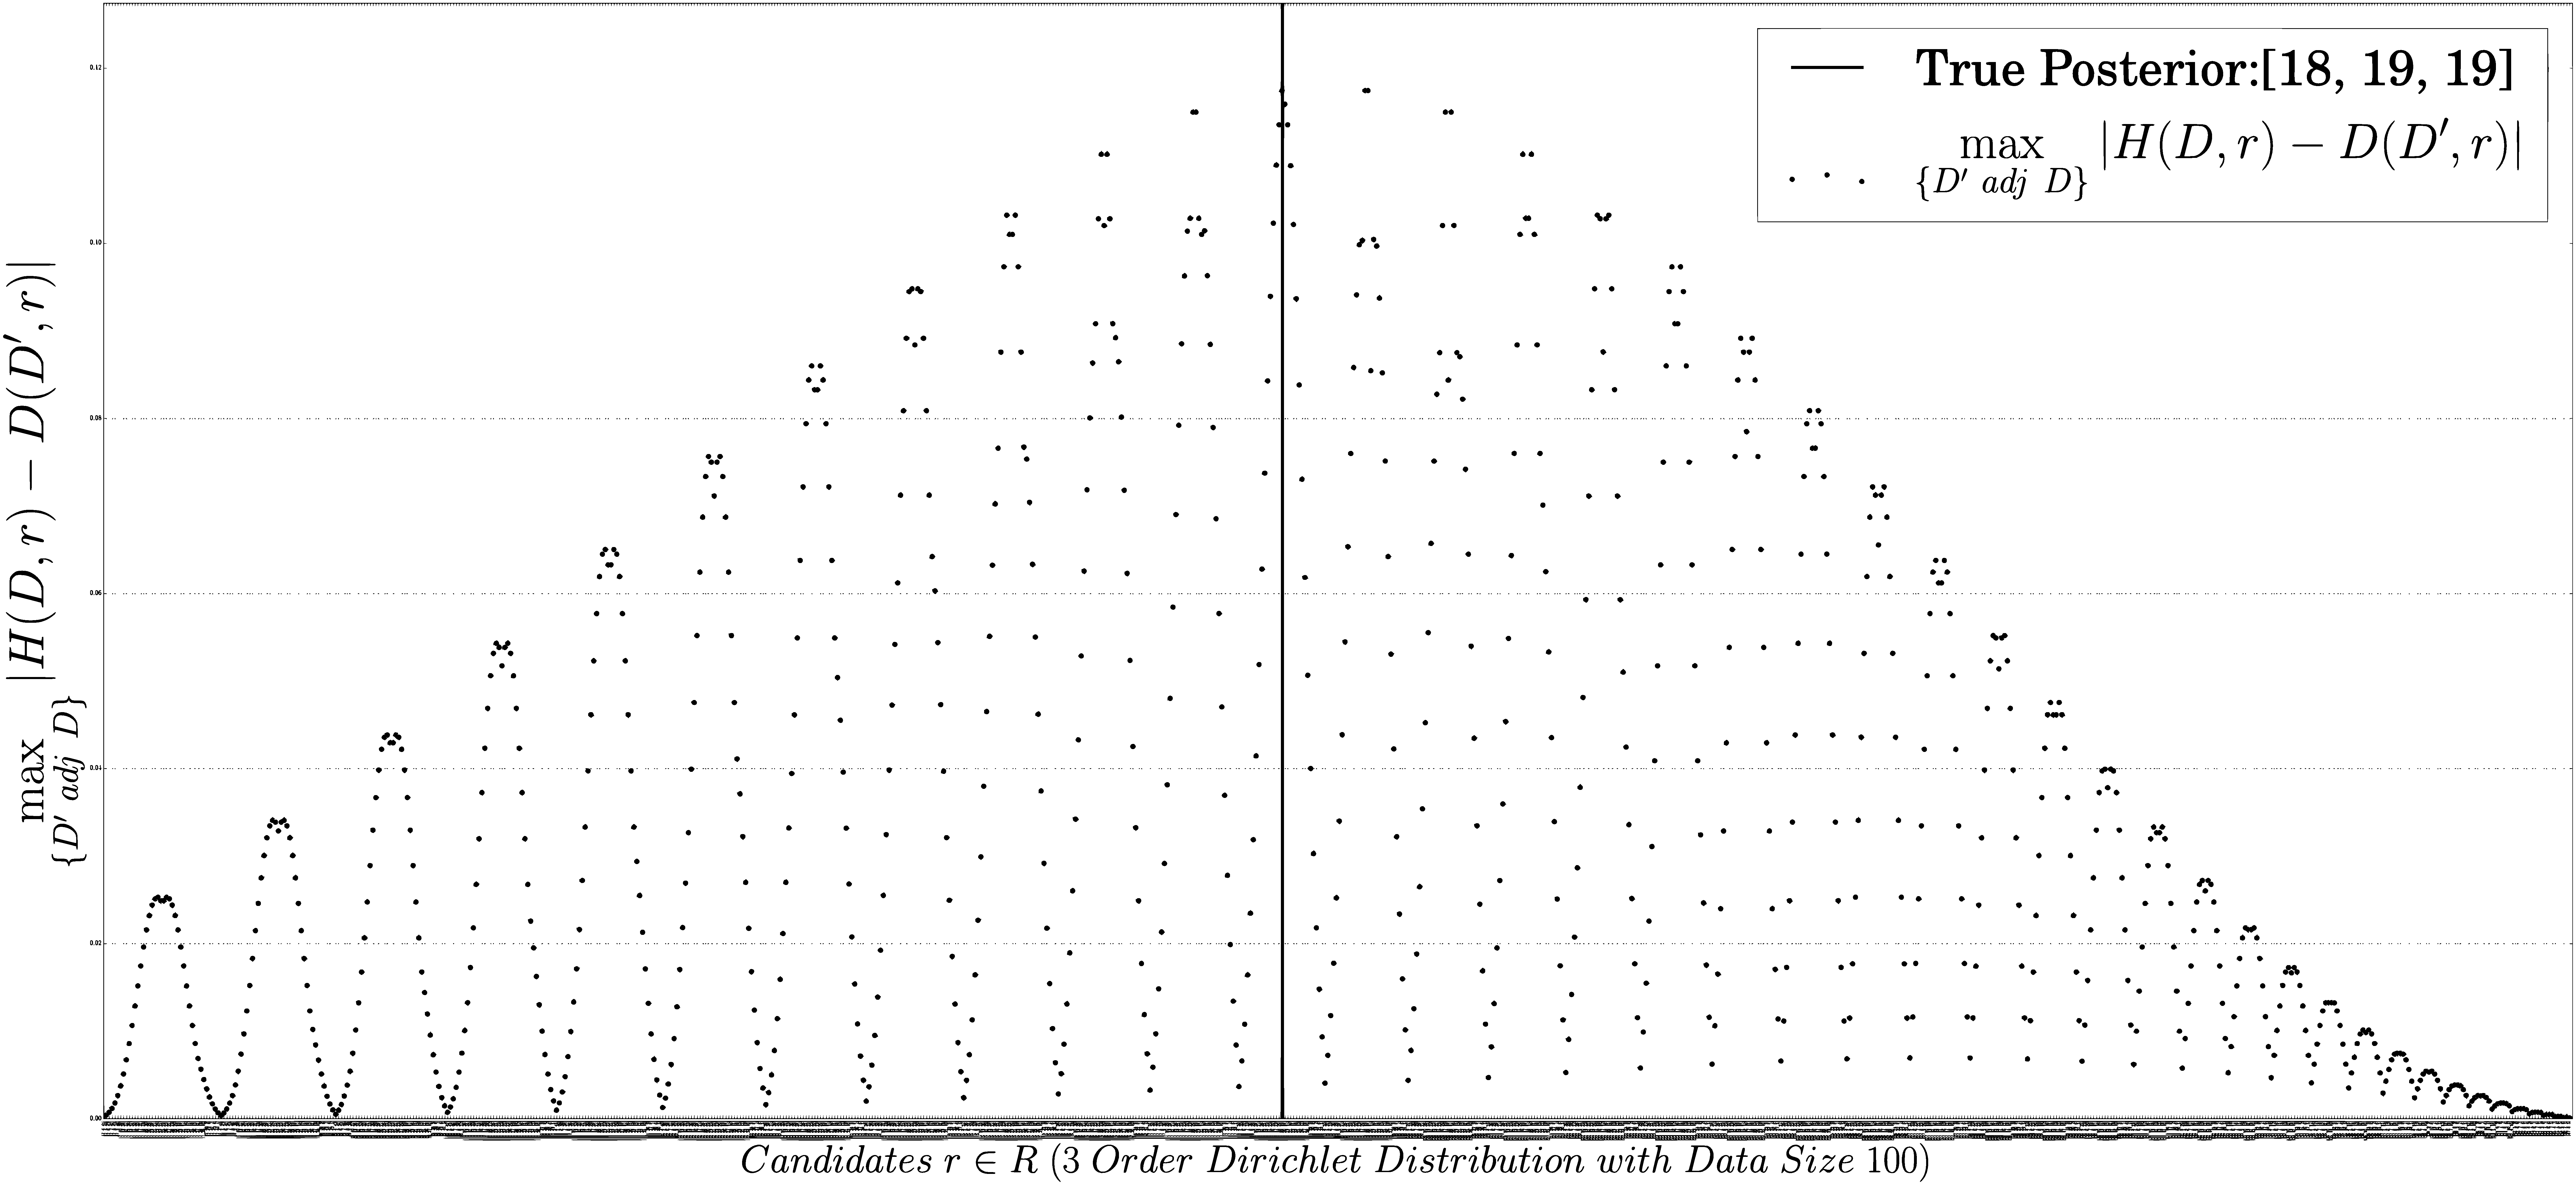
\includegraphics[width=0.45\textwidth]{efficiency.eps}
% \caption{Experimental Results for Finding the Local Sensitivity Efficiently}
% \label{fig_efficiency}
% \end{figure}

\subsection{Accuracy Evaluation}
\subsubsection{Theoretical Results}
In Fig. \ref{fig_theory} and \ref{fig_theory_epsilon}, we plot on the x-axis the Hellinger distance from the true posterior and on the y-axis the theoretical probabilities of outputting the candidates with that distance under the different mechanisms. We consider \emph{balanced} data sets, which means that in the Beta-Binomial model (Figure \ref{subfig_theory_2d}) the datasets will consist of 50\% 1s and the rest 0s, while for the
Dirichelet-Multinomial (Figure  \ref{subfig_theory_3d})
the data will be split in the $k=3$ bins with perecentages of: 33\%, 33\% and 34\% in 3 dimensionality. Same concept in 4 dimensionality.

We consider 5 mechanisms in our comparison experiments, including the Laplace mechanism ($\lapmech$), improved Laplace mechanism ($\ilapmech$),
standard exponential mechanism ($\mathsf{expMech}$),
non private exponential mechanism ($\lexpmech$) and the newly designed mechanisms ($\hexpmech$ with $\gamma$ sensitivity achieving $\epsilon-$dp).

\begin{figure}
\begin{center}
\centering
  \subfigure[2 dimensions, data size $600$]{
    \includegraphics[width=0.22\textwidth]{theory_2d.eps}
  \label{subfig_theory_2d}
  }
  \subfigure[3 dimensions, data size $600$]{
    \includegraphics[width=0.22\textwidth]{theory_3d.eps}
  \label{subfig_theory_3d}
  }
\caption{The theory probabilities of outputting candidates in certain distance from true posterior, with balanced data set and parameters $\epsilon = 1.0$}
\label{fig_theory}
\end{center}
\end{figure}

Candidates of smaller distance from true posterior are considered to be good results, which can result in good accuracy. From Fig. \ref{fig_theory}, it can be derived that all these mechanisms (except standard exponential mechanism $\expmech$ in green line) can output good results with larger probability. The $\lexpmech$ can output good results with higher probability than others, but $\lexpmech$ is non private. For these are $\epsilon -$differentially private, the improved laplace mechanism $\ilapmech$ with $\ell_1$ norm metric can produce good results with higher probability, i.e., perform better in terms of accuracy than others. As the dimension increases from 2 to 3, mechanisms' behavior remain the same.

\begin{figure}
\begin{center}
\centering
  \subfigure[data size 1000]{
    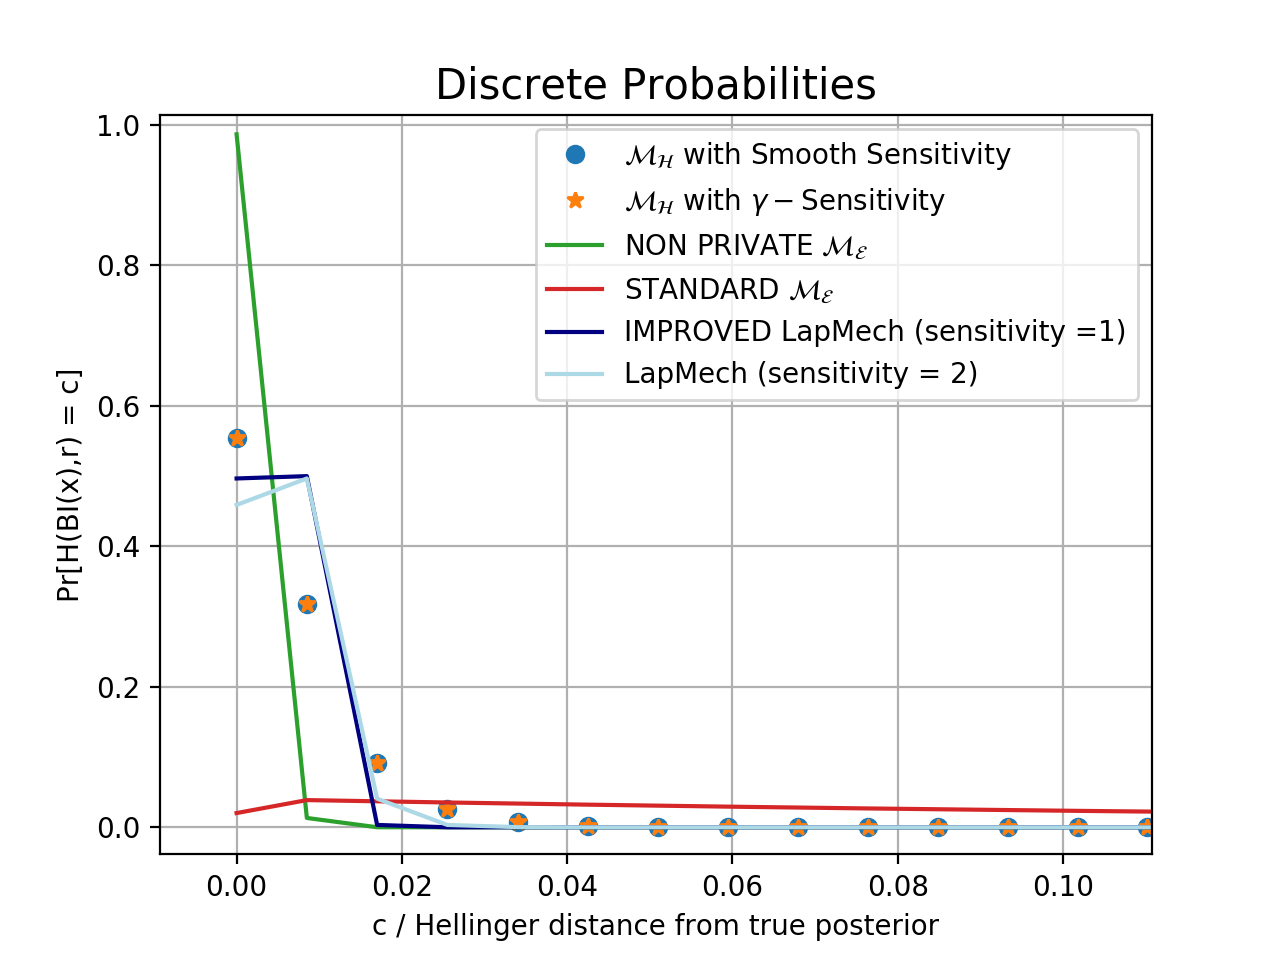
\includegraphics[width=0.22\textwidth]{epsilon5_2d_1000.eps}
  \label{subfig_theory_2d}
  }
  \subfigure[data size 10000]{
    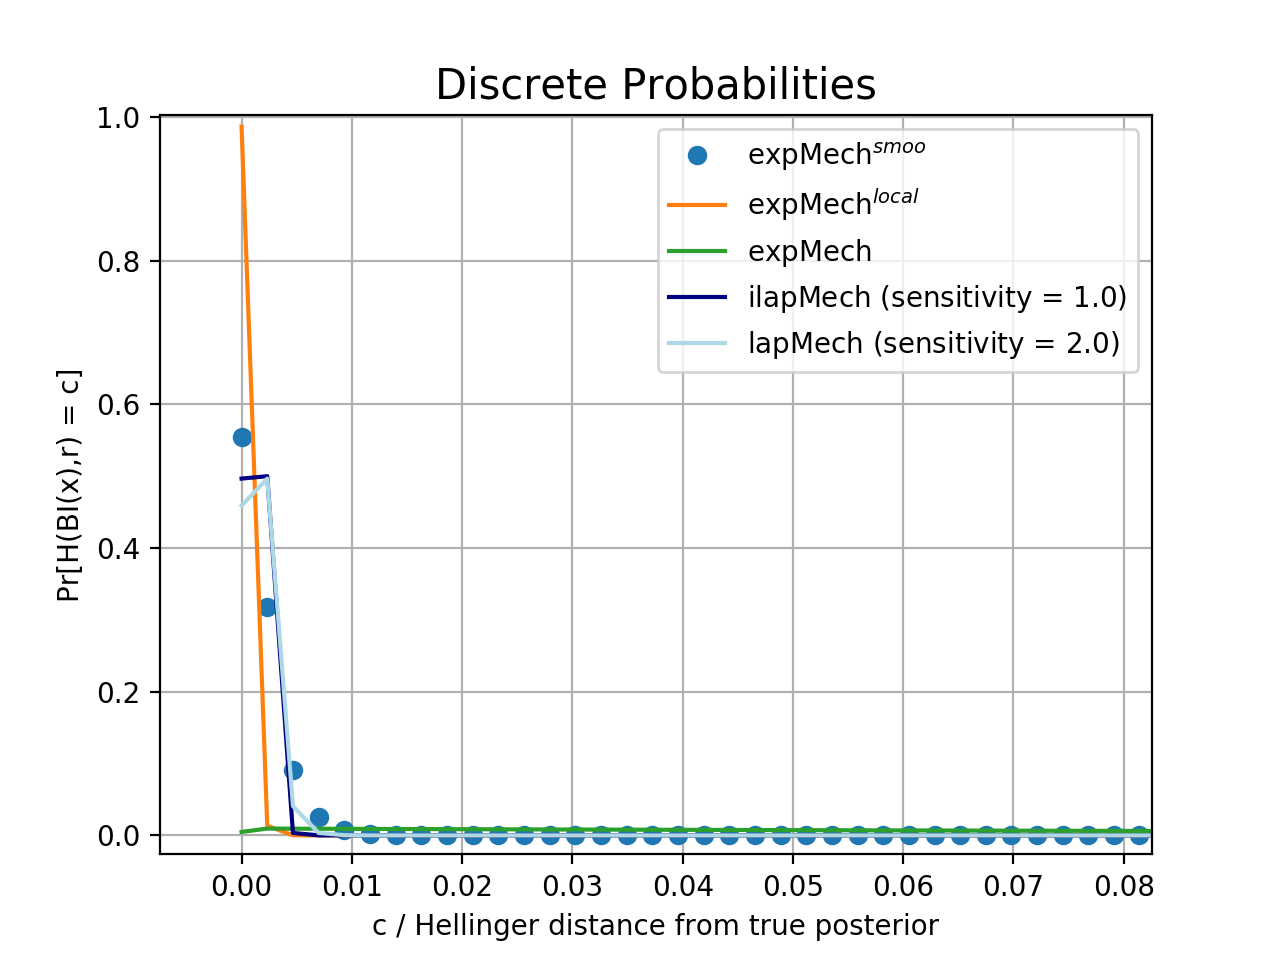
\includegraphics[width=0.22\textwidth]{epsilon5_2d_10000.eps}
  \label{subfig_theory_3d}
  }
\caption{The theory probabilities of outputting candidates in certain distance from true posterior, with balanced data set and parameters $\epsilon = 5.0$, in 2 dimensions}
\label{fig_theory_epsilon}
\end{center}
\end{figure}

Increasing the privacy bound $\epsilon$, we get theoretical results as in Fig. \ref{fig_theory_epsilon} in 2 dimensions. The $\lexpmech$ is still the one with the best accuracy, but it is non-private. However, the $\lapmech$ and $\ilapmech$ having the similar performance, and $\hexpmech$ can produce the correct posterior with higher probability than the others. And the standard exponential mechanism $\expmech$ is still the worst one.


\subsubsection{Experimental Results}
\label{subsec_vs_variables}

In this section, we evaluate the accuracy of the mechanisms defined in
Section (\ref{sec_mechs}) w.r.t. data sizes and dimensions by experimenting on real data sets.
Every plot is an average over 1000 runs. In all the experiments we set
$\epsilon = 1.0$.

\noindent In the following some of the plots show
mean error as a function of the datasize while one
is a whiskers-plot where the y-axis shows the average
accuracy (or equivalently, the error) of the mechanisms, and the x-axis, instead shows
different balanced priors used. The boxes extend from the lower to the upper quartile values
of the data, with a line at the median. A notch on the box around the
median is also drawn to give a rough guide to the significance of
difference of medians; The whiskers extend from the box to show the
range of the data. 
% A blue box in the plots represents the $\hexpmech$'s behavior-- where the sensitivity is calibrated
% w.r.t Hellinger distance-- while the green box next to
% it represents the performance of a variation of the basic Laplace
% mechanism $\lapmech$, and red one is $\ilapmech$ presented in Section (\ref{sec_mechs}) with the same
% settings: that is $\epsilon$, data, prior. The variation
% considered performs a postprocessing on the released parameters so
% that they are consistent. For instance when the sum of the noised
% parameters is greater than $n$ we will truncate them so that they sum
% up to $n$.

% \paragraph{Increasing data size with balanced datasets}
% \label{subsubsec_vs_datasize}


% \begin{figure}[ht]
% \begin{center}
% \centering
% \subfigure[Increasing data size with prior $\betad(1,1)$, balanced datasets and parameters $\epsilon = 1.0$]
% { \includegraphics[width=0.35\textwidth]{sampling_2d.eps}
% \label{fig_vs_datasize_2d}
% }

% \subfigure[Increasing data size with $\dirichlet{1,1,1}$ prior distribution, balanced datasets and parameters $\epsilon = 1.0$]
% {
%   \includegraphics[width=0.35\textwidth]{sampling_3d.eps} 
%   \label{fig_vs_datasize_3d}
% }
% \subfigure[Increasing data size with $\dirichlet{1,1,1,1}$ prior distribution, balanced datasets and parameters $\epsilon = 1.0$]
% {
%   \includegraphics[width=0.35\textwidth]{sampling_4d.eps} 
%   \label{fig_vs_datasize_4d}
% }
% \end{center}
% \end{figure}

% In Figures \ref{fig_vs_datasize_2d}, \ref{fig_vs_datasize_3d} and \ref{fig_vs_datasize_4d} we still consider \emph{balanced} data sets
% of observations. The results show that when the data size increases, the average errors of
% $\hexpmech$, $\lapmech$ and $\ilapmech$ decrease. For small datasets,
% i.e with size less $300$ in the case of Beta-Binomial models, the Laplace mechanisms outperform $\hexpmech$.
% But for bigger data sets, that is, bigger than $300$, or as in Figure \ref{fig_vs_datasize_2d} where
% we considered data sets of the order of 15 thousands elements,
% the $\hexpmech$ outperforms the $\lapmech$, and asymptotically approaches the improved Laplace mechanism $\ilapmech$.
% Similar experimental tendencies were obtained for the Dirichlet-multinomial model (Figure \ref{fig_vs_datasize_3d} and \ref{fig_vs_datasize_4d}).


\paragraph{Experiments on Real Data Sets in Beta-binomial Model}
We use four real data sets from UCI Machine Learning repository\footnote{https://archive.ics.uci.edu/ml/datasets.html}. Each data set contains 1 binary variable, which applys our Beta-binomial model. By setting the prior distribution as $\betad(1,1)$, we apply our 5 private inference algorithms on them to derive the underlining distribution of these data. The first data set is the SHARING BIKE data, where $0$ means user use sharing bike at workday and $1$ stands for weekend. The second and third data set the THERAPY data, where $1$ means patient with disease is cured and $1$ means not. The forth data set is the BADGE data, $1$ means people with badge and $0$ means without badge. The size of the four data set are $731, 90, 294, 90$. The accuracy are shown in Figure \ref{fig_real_2d}.
\begin{figure}
\centering
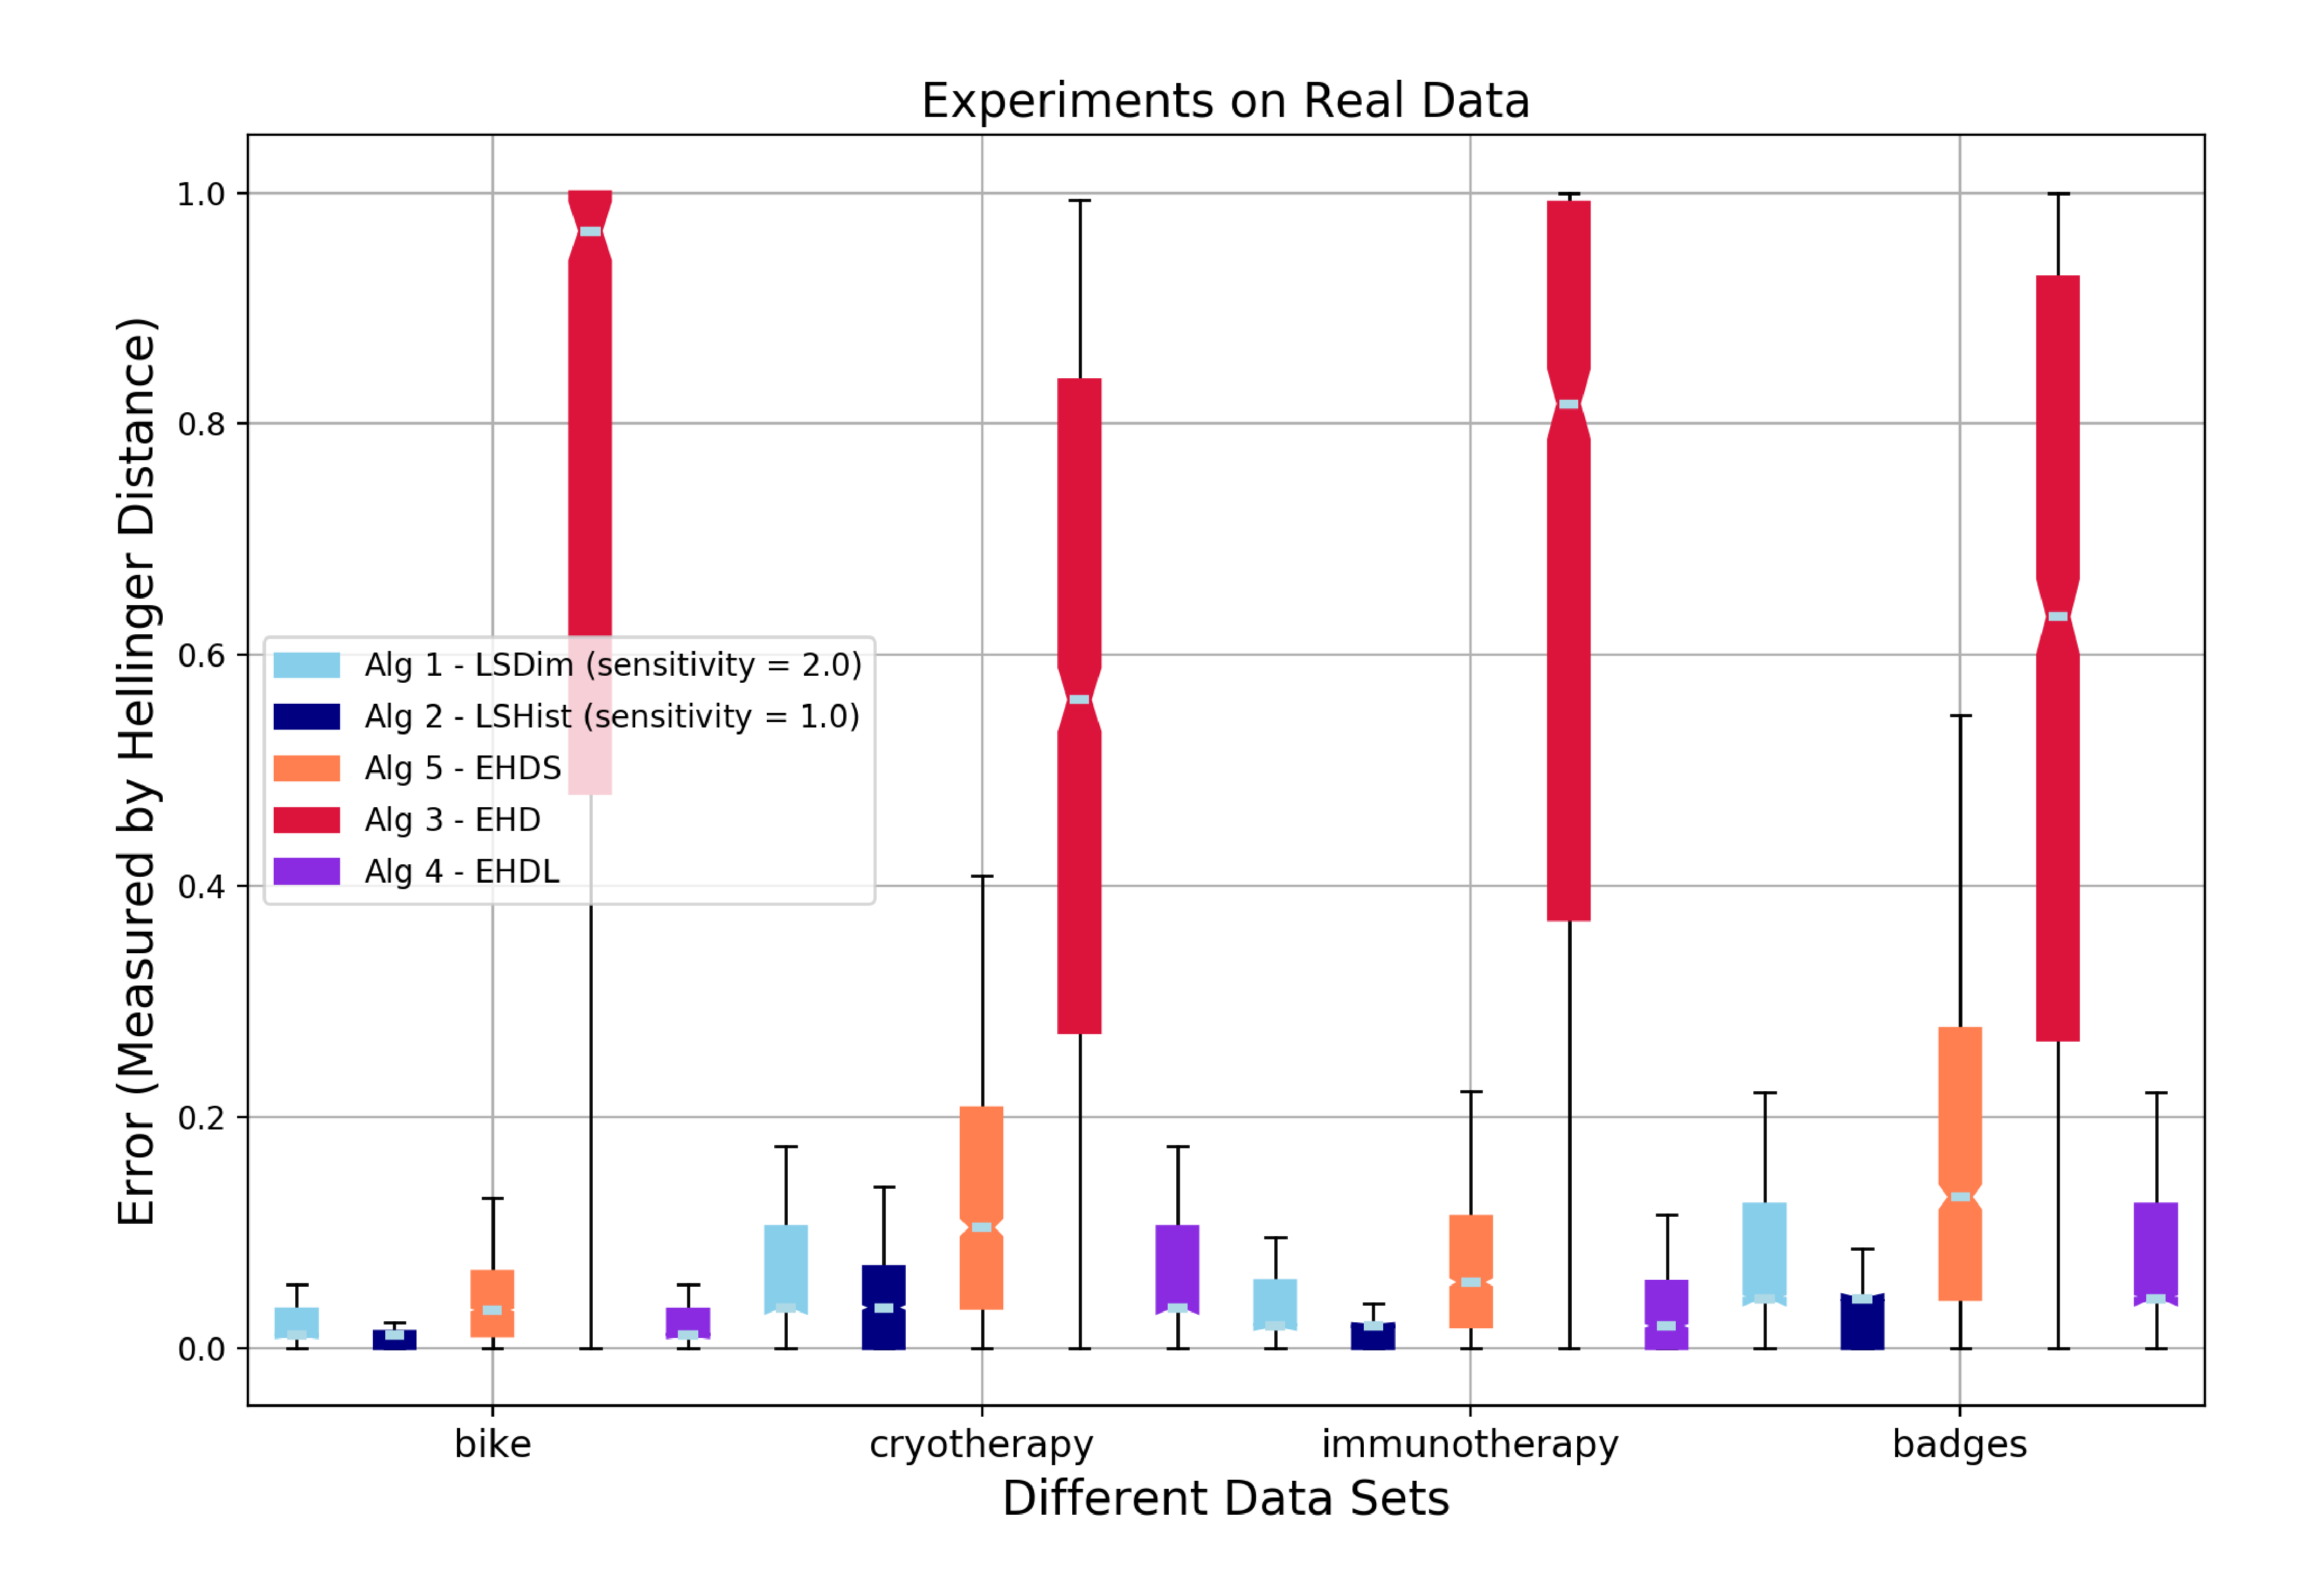
\includegraphics[width=0.35\textwidth]{realdata.eps}
\caption{Accuracy on Real Data Sets, with $\epsilon = 1.0$}
\label{fig_real_2d}
\end{figure}


\paragraph{Experiments on Real Data Sets in Dirichlet-multinomial Model}
We use three real data sets from the same repository repository. Each data set contains 1 category variable of 3 dimensions ($|\mathcal{X}| = 3$), which applys our 3 dimension Dirichlet-multinomial model. By setting the prior distribution as $\dirichlet{1,1,1}$, we apply our 5 private inference algorithms on them to derive the underlining distribution of these data. The first data set is the SHARING BIKE data, where $0$ means user use sharing bike at workday and $1$ stands for weekend. The second and third data set the THERAPY data, where $1$ means patient with disease is cured and $1$ means not. The forth data set is the BADGE data, $1$ means people with badge and $0$ means without badge. The size of the four data set are $731, 90, 90$. The accuracy are shown in Figure \ref{fig_real_3d}.
\begin{figure}
\centering
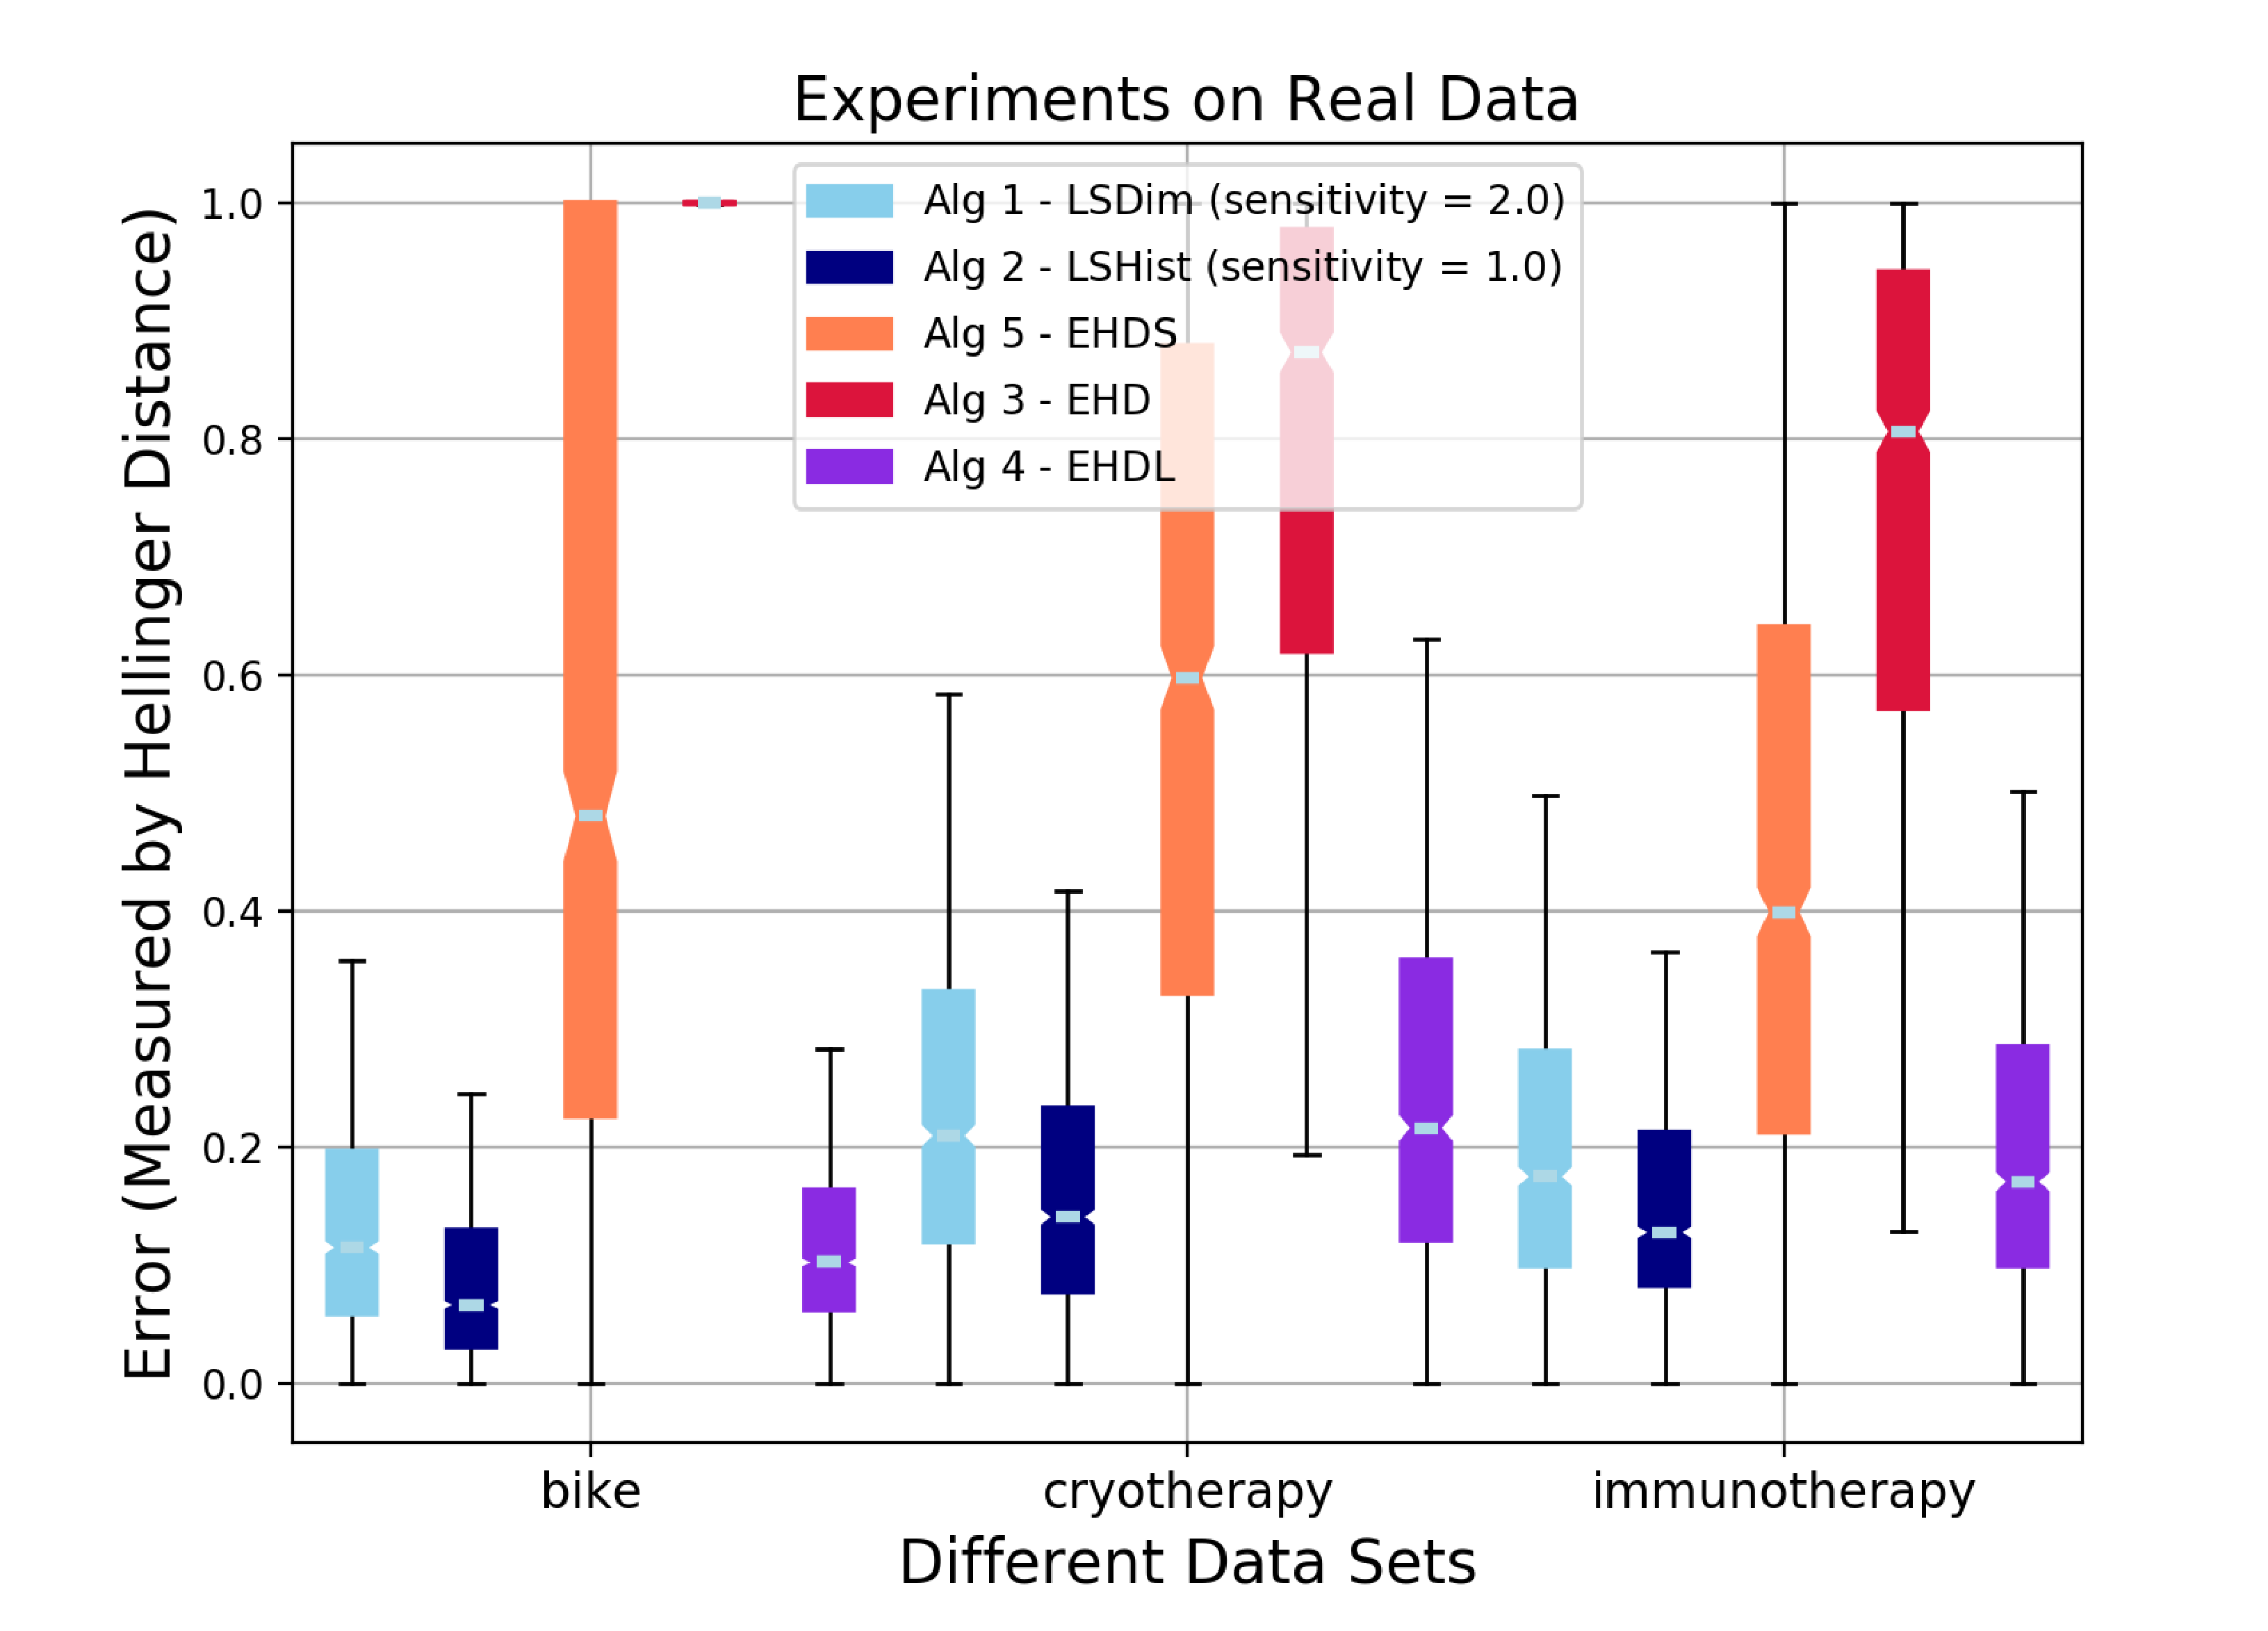
\includegraphics[width=0.35\textwidth]{realdata_3d.eps}
\caption{Accuracy on Real Data Sets, with $\epsilon = 1.0$}
\label{fig_real_3d}
\end{figure}


\subsection{Privacy Evaluation}
\label{subsec_experiment_privacy}
In order to see our privacy behavior, we study the accurate epsilon under concrete cases in this section. The $(\epsilon, \delta)$ - differential privacy we proved in Sec. \ref{sec_ehds} is just an upper bound, we concrete $\epsilon$ should be smaller than upper bound in our exponential mechanism. We calculate the concrete privacy value in following ways wrt. the data size, and obtain plots in Fig. \ref{fig_privacy}.

\begin{figure}
\begin{center}
\centering
    \includegraphics[width=0.35\textwidth]{privacyloss.eps}
\caption{Actual privacy loss of different data size when privacy bound $\epsilon = 1.0$ in 2 dimensions, prior:$\betad(1,1)$ and balanced data}
\label{fig_privacy}
\end{center}
\end{figure}

$\epsilon = 1.0$ is a privacy upper bound, we can observe that the concrete $\epsilon$ values are smaller than the upper bound. That is to say, we achieved a higher privacy level than expected. 


\section{Conclusion}
From what we have seen in the previous sections we can obtain following conclusions. We explored the design space of the mechanisms for differentially privacy Bayesian inference, by considering different metrics and different algorithms.
\begin{itemize}
  \item The accuracy can change a lot when considering different metrics and using different sensitivity values.
  \item Different algorithms have different performance w.r.t. different aspect. From the experimental results, Laplace mechanism family have a good efficiency and accuracy when using $\ell_1$ norm metric. But exponential mechanism family can be a good application when considering different metrics.
\end{itemize}


\bibliography{bysinfer}
\bibliographystyle{icml2019}


% \appendix

% \noindent \textbf{Theorem \ref{thm_gamma_smooth}.}
% \emph{
% Given data set $\dataobs$, the $\gamma -$smooth sensitivity of Bayesian inference process w.r.t. the Hellinger distance $S(\dataobs)$ satisfying:%\\
% whenever $\adj{\dataobs}{\dataobs'}$, 
% %\begin{equation}
% %\label{eq_gamma_smooth}
% $\frac{1}{S(\dataobs)} - \frac{1}{S(\dataobs')} \leq \gamma$.
% }

% \begin{proof}
% of Theorem. \ref{thm_gamma_smooth}.\\
% For $\adj{\dataobs}{\dataobs'}$ and arbitrary $\dataobs'' \in \{0,1\}^{n}$:\\
% From Equation (\ref{eq_smooth}), we can get:
% \[
% \frac{1}{S(\dataobs)} 
%  = \min_{\dataobs'' \in \{0,1\}^{n}}\bigg \{ \frac{1}{LS(\dataobs'')} +\gamma \cdot d(\dataobs,\dataobs'') \bigg \}\\
% \]

% Since $d(\dataobs,\dataobs'') \leq d(\dataobs,\dataobs') + d(\dataobs',\dataobs'') \leq 1 + d(\dataobs',\dataobs'')$:

% \begin{equation*}
% \begin{split}
% & \leq \min_{\dataobs'' \in \{0,1\}^{n}}\bigg \{  \frac{1}{LS(\dataobs'')} +\gamma \cdot (1 + d(\dataobs',\dataobs'')) \bigg \}\\
% & = \min_{\dataobs'' \in \{0,1\}^{n}}\bigg \{
% \gamma + \frac{1}{LS(\dataobs'')} +\gamma \cdot d(\dataobs',\dataobs'')\bigg 
% \}\\
% & = \gamma + \min_{\dataobs'' \in \{0,1\}^{n}}\bigg \{
% \frac{1}{LS(\dataobs'')} +\gamma \cdot d(\dataobs',\dataobs'')\bigg
% \}\\
% & = \gamma + \frac{1}{S(\dataobs')}
% \end{split}
% \end{equation*}
% Then we can get:
% $\frac{1}{S(\dataobs)} - \frac{1}{S(\dataobs')} \leq \gamma.$
% \end{proof}


% \noindent \textbf{Lemma \ref{lem_loc_opt}.}
% \emph{
% \[
% LS(\dataobs) = \max\limits_{\dataobs' \in \datauni^n:\adj{\dataobs}{\dataobs'}} \hellinger(\bysinfer{\dataobs}, \bysinfer(\dataobs')).
% \]
% }

% \begin{proof} of Lemma \ref{lem_loc_opt}.\\
% For any $r \in \mathcal{R}$ and $\dataobs' \in \datauni^n$ with $\adj{\dataobs}{\dataobs'}$, we have
% \begin{align*}
% &\lvert \hellinger(\bysinfer{\dataobs}, r) - \hellinger(\bysinfer(\dataobs'), r)\rvert\\
% & = 
% \begin{cases}
% \hellinger(\bysinfer{\dataobs}, r) - \hellinger(\bysinfer(\dataobs'),r) & \text{positive case}\\
% \hellinger(\bysinfer(\dataobs'),r) - \hellinger(\bysinfer{\dataobs}, r) & \text{negative case}
% \end{cases}\\
% & \leq 
% \begin{cases}
% \hellinger(\bysinfer(\dataobs'), \bysinfer{\dataobs})+
% \hellinger(\bysinfer(\dataobs'), r) - \hellinger(\bysinfer(\dataobs'),r) & \\
% \hellinger(\bysinfer(\dataobs'), \bysinfer{\dataobs})+
% \hellinger(\bysinfer{\dataobs}, r) - \hellinger(\bysinfer{\dataobs}, r)&
% \end{cases}\\
% &= \hellinger(\bysinfer(\dataobs'), \bysinfer{\dataobs})
% \end{align*}
% The equality holds if $r = \bysinfer{\dataobs}$ or $r = \bysinfer(\dataobs')$.
% Hence, we conclude the statement of this lemma.
% \end{proof}



% \noindent \textbf{ Lemma \ref{lem_hexpmech_privacy}. } 
% \emph{
% $\hexpmech$ is $\epsilon$-differential privacy by setting $\gamma = 1.0$.
% }

% \begin{proof} of Lemma \ref{lem_hexpmech_privacy}.\\
%   By Definition \ref{def_epsilon_dp}, to proof Lemma \ref{lem_hexpmech_privacy}, we need to prove:\\
%   For any $\adj{\dataobs}{\dataobs'} \in \mathcal{X}$ and any beta distribution $r$:
%   \begin{equation*}
%   \hexpmechPr{\dataobs}{z = r} \leq e^{\epsilon} \hexpmechPr{\dataobs'}{z = r}. 
%   \end{equation*}
%   By definition \ref{def_smoo_2}:
%   \begin{equation*}
%   \begin{split}
%   \hexpmechPr{\dataobs}{z = r} 
%   & = \frac {\exp\big(\frac{-\epsilon\cdot\ux{r}}{4\cdot S(\dataobs)}\big)}{\unomalizer{\dataobs}} \\
%   & = \frac {\exp\big(
%   \frac{-\epsilon\cdot(\ux{r} + \uxadj{r} - \uxadj{r})}{4\cdot S(\dataobs)}
%   \big)}
%   {\unomalizer{\dataobs}} \\
%   & = \frac {\exp\big(
%   \frac{-\epsilon\cdot(\uxadj{r})}{4\cdot S(\dataobs)}
%   \big)}
%   {\unomalizer{\dataobs}}
%   \\
%   & \cdot \exp\big( \frac{\epsilon\cdot(\uxadj{r} - \ux{r})}{4\cdot S(\dataobs)} \big)\\
%   \end{split}
%   \end{equation*}
%   Because $S(\dataobs) \geq LS(\dataobs) \geq (\uxadj{r} - \ux{r})$:
%   \begin{equation*}
%   \begin{split}
%   & \leq \frac {\exp\big(
%   \frac{-\epsilon\cdot(\uxadj{r})}{4\cdot S(\dataobs)}
%   \big)}
%   {\unomalizer{\dataobs}}
%   \cdot \exp\big( \frac{\epsilon}{4} \big) \\
%   & = \exp\big( \frac{\epsilon}{4} \big) \cdot 
%   \frac {
%   \exp
%   \big(
%   \frac{-\epsilon\cdot(\uxadj{r})}{4\cdot S(\dataobs)}
%   \big)
%   } 
%   {\unomalizer{\dataobs}}\\
%   & \cdot \exp
%   \big(
%   \frac{\epsilon\cdot(\uxadj{r})}{4\cdot S(\dataobs')}
%   \big)
%   \exp
%   \big(
%   \frac{-\epsilon\cdot(\uxadj{r})}{4\cdot S(\dataobs')}
%   \big)\\
%   & = \exp\big( \frac{\epsilon}{4} \big) \cdot 
%   \frac {
%   \exp
%   \big(
%   \frac{-\epsilon\cdot(\uxadj{r})}{4\cdot S(\dataobs')}
%   \big)
%   } 
%   {\unomalizer{\dataobs}}\\
%   & \cdot \exp
%   \big(
%   \frac{\epsilon\cdot(\uxadj{r})}{4}(\frac{1}{S(\dataobs')} - \frac{1}{S(\dataobs)})
%   \big)\\
%   \end{split}
%   \end{equation*}
  
%   Because $\uxadj{r} = \hellinger(\bysinfer(\dataobs'), r) \leq 1$:
%   \begin{equation*}
%   \begin{split}
%   & \leq \exp\big( \frac{\epsilon}{4} \big) \cdot 
%   \frac {
%   \exp
%   \big(
%   \frac{-\epsilon\cdot(\uxadj{r})}{4\cdot S(\dataobs')}
%   \big)
%   } 
%   {\unomalizer{\dataobs}}\\
%   & \cdot \exp
%   \big(
%   \frac{\epsilon}{4}(\frac{1}{S(\dataobs')} - \frac{1}{S(\dataobs)})
%   \big)\\
%   \end{split}
%   \end{equation*}

%   Because the property of $\gamma -$smooth sensitivity: $\frac{1}{S(\dataobs')} - \frac{1}{S(\dataobs)} \leq \gamma$:  
%   \begin{equation*}
%   \begin{split}
%   & \leq \exp\big( \frac{\epsilon}{4} \big) \cdot 
%   \frac {
%   \exp
%   \big(
%   \frac{-\epsilon\cdot(\uxadj{r})}{4\cdot S(\dataobs')}
%   \big)
%   } 
%   {\unomalizer{\dataobs}}
%   \exp
%   \big(
%   \frac{\epsilon}{4} \cdot \gamma
%   \big)\\
%   & = \exp\big( \frac{\epsilon}{4} + \frac{\epsilon}{4} \cdot \gamma\big) \cdot 
%   \frac {
%   \exp
%   \big(
%   \frac{-\epsilon\cdot(\uxadj{r})}{4\cdot S(\dataobs')}
%   \big)
%   } 
%   {\unomalizer{\dataobs}}\\
%   \end{split}
%   \end{equation*}

%   Doing the same transformation in the denominator:
%   \begin{equation*}
%   \begin{split}
%   & = \exp\big( \frac{\epsilon}{4} + \frac{\epsilon}{4} \cdot \gamma\big) \cdot 
%   \frac {
%   \exp
%   \big(
%   \frac{-\epsilon\cdot(\uxadj{r})}{4\cdot S(\dataobs')}
%   \big)
%   } 
%   {
%   \sum_{r'\in \candidateset} 
%   \exp 
%   \big(
%   \frac{-\epsilon\cdot(\ux{r'} + \uxadj{r'} - \uxadj{r'})}{4 \cdot S(\dataobs)}
%   \big)
%   }\\
%   & = \exp\big( \frac{\epsilon}{4} + \frac{\epsilon}{4} \cdot \gamma\big) \\
%   & \cdot 
%   \frac {
%   \exp
%   \big(
%   \frac{-\epsilon\cdot(\uxadj{r})}{4\cdot S(\dataobs')}
%   \big)
%   } 
%   {
%   \sum_{r'\in \candidateset} 
%   \exp 
%   \big(
%   \frac{-\epsilon\cdot(\uxadj{r'}}{4 \cdot S(\dataobs)}
%   \big)
%   \exp 
%   \big(
%   \frac{-\epsilon\cdot(\ux{r'} - \uxadj{r'})}{4 \cdot S(\dataobs)}
%   \big)
%   }\\
%   \end{split}
%   \end{equation*}

%   Because $S(\dataobs) \geq LS(\dataobs) \geq (\ux{r} - \uxadj{r})$ $\implies$ $ \frac{-\epsilon\cdot(\ux{r'} - \uxadj{r'})}{4 \cdot S(\dataobs)} \geq \frac{-\epsilon}{4}$:
%   \begin{equation*}
%   \begin{split}
%   & \leq \exp\big( \frac{\epsilon}{4} + \frac{\epsilon}{4} \cdot \gamma\big) \cdot 
%   \frac {
%   \exp
%   \big(
%   \frac{-\epsilon\cdot(\uxadj{r})}{4\cdot S(\dataobs')}
%   \big)
%   } 
%   {
%   \sum_{r'\in \candidateset} 
%   \exp 
%   \big(
%   \frac{-\epsilon\cdot(\uxadj{r'}}{4 \cdot S(\dataobs)}
%   \big)
%   \exp 
%   \big(
%   \frac{-\epsilon}{4}
%   \big)
%   }\\
%   & = \exp\big( \frac{\epsilon}{4} + \frac{\epsilon}{4} \cdot \gamma\big) \cdot 
%   \frac {
%   \exp
%   \big(
%   \frac{-\epsilon\cdot(\uxadj{r})}{4\cdot S(\dataobs')}
%   \big)
%   } 
%   {
%   \sum_{r'\in \candidateset} 
%   \exp 
%   \big(
%   \frac{-\epsilon\cdot(\uxadj{r'}}{4 \cdot S(\dataobs)}
%   \big)
%   }\\
%   & \cdot 
%   \frac{1}
%   {
%   \exp 
%   \big(
%   \frac{-\epsilon}{4}
%   \big)
%   \exp
%   \big(
%   \frac{\epsilon\cdot(\uxadj{r'})}{4\cdot S(\dataobs')}
%   \big)
%   \exp
%   \big(
%   \frac{-\epsilon\cdot(\uxadj{r'})}{4\cdot S(\dataobs')}
%   \big)
%   }\\
%   & = \exp\big( \frac{\epsilon}{4} + \frac{\epsilon}{4} \cdot \gamma\big) \cdot 
%   \frac {
%   \exp
%   \big(
%   \frac{-\epsilon\cdot(\uxadj{r})}{4\cdot S(\dataobs')}
%   \big)
%   } 
%   {
%   \sum_{r'\in \candidateset} 
%   \exp 
%   \big(
%   \frac{-\epsilon\cdot(\uxadj{r'}}{4 \cdot S(\dataobs')}
%   \big)}\\
%   & \cdot\frac{1}{
%   \exp 
%   \big(
%   \frac{-\epsilon}{4}
%   \big)
%   \exp
%   \big(
%   \frac{- \epsilon\cdot(\ux{r'})}{4}
%   (\frac{1}{S(\dataobs)}
% -
%   \frac{1}{S(\dataobs')})
%   \big)
%   }
%   \end{split}
%   \end{equation*}

%   Because $\uxadj{r} = \hellinger(\bysinfer(\dataobs'), r) \leq 1$ $\implies$ $\frac{- \epsilon\cdot(\ux{r'})}{4} \geq  \frac{-\epsilon}{4}$:
%   \begin{equation*}
%   \begin{split}
%   & \leq \exp\big( \frac{\epsilon}{4} + \frac{\epsilon}{4} \cdot \gamma\big) \cdot 
%   \frac {
%   \exp
%   \big(
%   \frac{-\epsilon\cdot(\uxadj{r})}{4\cdot S(\dataobs')}
%   \big)
%   } 
%   {
%   \sum_{r'\in \candidateset} 
%   \exp 
%   \big(
%   \frac{-\epsilon\cdot(\uxadj{r'}}{4 \cdot S(\dataobs')}
%   \big)}\\
%   & \cdot \frac{1}{
%   \exp 
%   \big(
%   \frac{-\epsilon}{4}
%   \big)
%   \exp
%   \big(
%   \frac{- \epsilon}{4}
%   (\frac{1}{S(\dataobs)}
% -
%   \frac{1}{S(\dataobs')})
%   \big)
%   }\\
%   \end{split}
%   \end{equation*}

%   Because the property of $\gamma -$ smooth sensitivity: $\frac{1}{S(\dataobs)} - \frac{1}{S(\dataobs')} \leq \gamma$ $\implies$
%   $\frac{- \epsilon}{4}
%   (\frac{1}{S(\dataobs)}-
%   \frac{1}{S(\dataobs')}) \geq \frac{- \epsilon}{4} \cdot \gamma$
%   \begin{equation*}
%   \begin{split}
%   & \leq \exp\big( \frac{\epsilon}{4} + \frac{\epsilon}{4} \cdot \gamma\big) \cdot 
%   \frac {
%   \exp
%   \big(
%   \frac{-\epsilon\cdot(\uxadj{r})}{4\cdot S(\dataobs')}
%   \big)
%   } 
%   {
%   \sum_{r'\in \candidateset} 
%   \exp 
%   \big(
%   \frac{-\epsilon\cdot(\uxadj{r'}}{4 \cdot S(\dataobs')}
%   \big)
%   \exp 
%   \big(
%   \frac{-\epsilon}{4}
%   \big)
%   \exp
%   \big(
%   \frac{- \epsilon}{4} \cdot \gamma
%   \big)
%   }\\
%   & = \exp\big( \frac{\epsilon}{4} + \frac{\epsilon}{4} \cdot \gamma\big) \cdot 
%   \frac {
%   \exp
%   \big(
%   \frac{-\epsilon\cdot(\uxadj{r})}{4\cdot S(\dataobs')}
%   \big)
%   } 
%   {
%   \sum_{r'\in \candidateset} 
%   \exp 
%   \big(
%   \frac{-\epsilon\cdot(\uxadj{r'}}{4 \cdot S(\dataobs')}
%   \big)
%   \exp 
%   \big(
%   \frac{-\epsilon}{4} +   \frac{- \epsilon}{4} \cdot \gamma
%   \big)
%   }\\
%   & = e^{( \frac{\epsilon}{2} + \frac{\epsilon}{2} \cdot \gamma )} \cdot 
%   \frac {
%   \exp
%   \big(
%   \frac{-\epsilon\cdot(\uxadj{r})}{4\cdot S(\dataobs')}
%   \big)
%   } 
%   {
%   \unomalizer{\dataobs'}
%   }\\
%   & = e^{( \frac{\epsilon}{2} + \frac{\epsilon}{2} \cdot \gamma )} \cdot   \hexpmechPr{\dataobs'}{z = r}
%   \end{split}
%   \end{equation*}

%   Given $\gamma = 1$, $\epsilon - $differential privacy can be achieved by $\hexpmech$.


% \end{proof}


% \noindent \textbf{ Lemma \ref{lem_acc_lap}.}
% \emph{
% Given $Y \thicksim \lap{0}{b}$, the accuracy bound developed for $\lapmech$ is:
% \begin{align*}
% &
% \lapmechPr{\dataobs}{
% \begin{aligned}
% \lefteqn{\hellinger(\bysinfer{\dataobs}, z )}\\ 
% &= \hellinger(\betad(\alpha, \beta), \betad(\alpha + t, \beta - t)
% \end{aligned}
% }
% \\
% &\qquad = 
% \begin{cases}
% \frac{1}{2} (e^{- \frac{\epsilon (t)}{\Delta }} - e^{- \frac{\epsilon (t + 1)}{\Delta }}) &  t \geq 0\\
% \frac{1}{2} (e^{\frac{\epsilon (t + 1)}{\Delta }} - e^{\frac{\epsilon (t)}{\Delta }}) & t < 0
% \end{cases}
% \end{align*}
% where $\betad(\alpha, \beta)$ is the true posterior distribution, i.e., $\bysinfer{\dataobs} = \betad(\alpha, \beta)$, and $r_L$ be the posterior produced by Laplace mechanism, i.e., $z = \betad(\alpha + \lfloor Y \rfloor, \beta - \lfloor Y \rfloor)$.
% }

% \begin{proof} of Lemma \ref{lem_acc_lap}.\\
% Given $Y \thicksim \lap{0}{b}$, we have\cite{dwork2014algorithmic}:$\Pr[|Y| \geq t \cdot b] = e^{- t}.$\\
% Based on this, we get:$\Pr[|Y| \geq t] = e^{- \frac{t \epsilon}{\Delta }}$, where $Y \thicksim \lap{0}{\frac{\Delta }{\epsilon}}$ in our setting.

% Considering the post-processing (i.e., taking the floor value of $Y$) in $\lapmech$, we have:
% %\[
% %\Pr\big[\lfloor Y \rfloor = t\big] 
% %= \Pr[ t \leq Y < t + 1] 
% %= \frac{1}{2} (e^{- \frac{\epsilon (t)}{\Delta \bysinfer}} - e^{- \frac{\epsilon (t + 1)}{\Delta \bysinfer}}).
% %\]
% %when $t \geq 0$, and
% %\[
% %\Pr\big[\lfloor Y \rfloor = t\big] 
% %= \Pr[ t \leq Y < t + 1] 
% %= \frac{1}{2} (e^{\frac{\epsilon (t)}{\Delta \bysinfer}} - e^{\frac{\epsilon (t + 1)}{\Delta \bysinfer}}).
% %\]
% %when $t < 0$.
% \begin{align*}
% \Pr\big[\lfloor Y \rfloor = t\big]&= \Pr[ t \leq Y < t + 1]\\
% &= 
% \begin{cases}
% \frac{1}{2} (e^{- \frac{\epsilon (t)}{\Delta }} - e^{- \frac{\epsilon (t + 1)}{\Delta }}) &  t \geq 0\\
% \frac{1}{2} (e^{\frac{\epsilon (t)}{\Delta }} - e^{\frac{\epsilon (t + 1)}{\Delta }}) & t < 0
% \end{cases}
% \end{align*}

% Let $\betad(\alpha, \beta)$ be the true posterior distribution, i.e., $\bysinfer{\dataobs} = \betad(\alpha, \beta)$, and $r_L$ be the posterior produced by Laplace mechanism, i.e., $r_L = \betad(\alpha + \lfloor Y \rfloor, \beta - \lfloor Y \rfloor)$. By applying Hellinger distance in our case, we get:
% %$$
% %\begin{array}{rcl}
% %& \Pr\big[\hellinger(\bysinfer{\dataobs}, r_L ) 
% %= \hellinger(\betad(\alpha, \beta), \betad(\alpha + t, \beta - t)\big] \\
% %& =  \frac{1}{2} (e^{- \frac{\epsilon (t)}{\Delta \bysinfer}} - e^{- \frac{\epsilon (t + 1)}{\Delta \bysinfer}})\\
% %\end{array}
% %$$
% %when $t \geq 0$, and\\
% %$$
% %\begin{array}{rcl}
% %& \Pr\big[\hellinger(\bysinfer{\dataobs}, r_L ) 
% %= \hellinger(\betad(\alpha, \beta), \betad(\alpha + t, \beta - t)\big]\\
% %& = \frac{1}{2} (e^{\frac{\epsilon (t + 1)}{\Delta \bysinfer}} - e^{\frac{\epsilon (t)}{\Delta \bysinfer}}).
% %\end{array}
% %$$
% %when $t < 0$.\\
% \begin{align*}
% &
% \Pr\left[
% \begin{aligned}
% \lefteqn{\hellinger(\bysinfer{\dataobs}, r_L )}\\ 
% &= \hellinger(\betad(\alpha, \beta), \betad(\alpha + t, \beta - t)
% \end{aligned}
% \right]
% \\
% &\qquad = 
% \begin{cases}
% \frac{1}{2} (e^{- \frac{\epsilon (t)}{\Delta }} - e^{- \frac{\epsilon (t + 1)}{\Delta }}) &  t \geq 0\\
% \frac{1}{2} (e^{\frac{\epsilon (t + 1)}{\Delta }} - e^{\frac{\epsilon (t)}{\Delta }}) & t < 0
% \end{cases}
% \end{align*}

% Unfolding the Hellinger distance formula, we get:\\
%   \noindent \textbf{case: t is even}
%   \begin{align*}
%   &\Pr\left[
% \begin{aligned}\lefteqn{\hellinger(\bysinfer{\dataobs}, r_L )^2}\\
% &= 1 - \prod_{k = 0}^{\frac{t}{2} - 1}
%   \sqrt{1 - \frac{\frac{t}{2}}{a + k + \frac{t}{2}}}
%   \cdot\prod_{k = 1}^{\frac{t}{2}}
%   \sqrt{1 - \frac{\frac{t}{2}}{\beta - k}}
% \end{aligned}
% \right] \\
%   &\qquad = \frac{1}{2} (e^{- \frac{\epsilon (t)}{\Delta }} - e^{- \frac{\epsilon (t + 1)}{\Delta }})
%   \end{align*}
%   \noindent \textbf{case: t is odd}
%   let $t = 2 m + 1$
%   \begin{align*}
%   & \Pr\left[
%   \begin{aligned}\lefteqn{\hellinger(\bysinfer{\dataobs}, r_L )^2} \\
%   & =
%   1 - \frac{\Gamma(\alpha+\frac{1}{2})}{\Gamma(\alpha)} \cdot
% \frac{\Gamma(\beta - \frac{1}{2})}{\Gamma(\beta)}\\
% &\cdot 
%   \prod_{k = 0}^{m-1}
%   \sqrt{(1 + \frac{1}{2(\alpha + k)})
%   (1 + \frac{\frac{1}{2} - m}{(\alpha + m  + k)})
%   }\\ &\cdot 
%   \prod_{k = 1}^{m} 
%   \sqrt{(1 + \frac{1}{2(\beta - \frac{1}{2}- k)})(1 + \frac{\frac{1}{2} - m}{(\beta - \frac{1}{2}- k)})} \end{aligned}
% \right] \\
%    &\qquad = \frac{1}{2} (e^{- \frac{\epsilon (t)}{\Delta }} - e^{- \frac{\epsilon (t + 1)}{\Delta }})
%   \end{align*}

% \end{proof}

\end{document}

